\documentclass[12pt,a4paper]{report}

\usepackage{epcc}
\usepackage{graphics}
\usepackage{hyperref}
% \usepackage{mathtools}
\usepackage{amsmath}
\usepackage{float}

% This example file shows how a thesis can be laid out using Latex. It
% does not use any special local features so should be portable to other
% places.
% 
% When producing draft copies of a thesis you may want to print only
% selected pages of the thesis. To do this use the command
% 
% dvips -f -p 4 -n 3 myfile.dvi | lpr
% 
% where -p 4 means start printing at page 4 (ie the page that will be
% numbered 4, not necessarily the 4th page) and -n 3 means print 3 pages.
% This example will print pages 4, 5 and 6.
% 
% If you want to print the thesis and also save paper you can print more
% than one page on each sheet of paper. Use the command
% 
% dvips -f myfile.dvi | psnup -2 | lpr
% 
% to print 2 pages per sheet. psnup can take values 2, 4, 8, or 9.
%
% To produce a PDF version you can create a PostScript copy first
%
% dvips -f myfile.dvi > myfile.pdf
%
% and then convert it
%
% distill myfile.ps
%
% or you can go straight to PDF
%
% pdflatex myfile
%
% Note that pdflatex expects all included figures to be in PDF too. See
% the includegraphics command below.


% This document contains many cross-references and forward references,
% eg in constructing a table of contents, so Latex may need to be run
% twice to get all the references correct. If you need to run Latex twice
% you may get the warning:
% 
% LaTeX Warning: Label(s) may have changed. Rerun to get cross-refSerences right.


% the following 4 lines are the content of the smallmargins.sty file
% but including them explicitly makes this more portable.
%AC%\oddsidemargin=0.1in
%AC%\topmargin=-0.5in
%AC%\textheight=9in
%AC%\textwidth=6.25in

%AC%\parskip 10pt
%AC%\parindent 0in

\begin{document}

%AC%\pagestyle{myheadings}
%AC%\markright{D.~S.~Henty}

%\title{A Latex thesis example}
%\author{D.~S.~Henty}
%\date{\today}

%\maketitle

\pagenumbering{roman}

\title{Bayesian Inference Using Sequential Monte-Carlo Algorithm for Dynamic System Models}
\author{Chaolin Han}
\date{\today}

\makeEPCCtitle

\thispagestyle{empty}

\vspace{11cm}

\begin{center}

\large{MSc in High Performance Computing}

\large{The University of Edinburgh}

\large{Year of Presentation: 2020}

\end{center}

\newpage

\begin{abstract}
This is the bit where you summarise what is in your thesis.
\end{abstract}

\pagenumbering{roman}

\tableofcontents
\listoftables
\listoffigures

\begin{titlepage}
\vspace*{2in}
% an acknowledgements section is completely optional but if you decide
% not to include it you should still include an empty {titlepage}
% environment as this initialises things like section and page numbering.
\section*{Acknowledgements}

This template is a slightly modified version of the one developed by
Prof. Charles Duncan for MSc students in the Dept. of Meteorology. His
acknowledgement follows:

{\em This template has been produced with help from many former students who
have shown different ways of doing things. Please make suggestions for
further improvements.}

\end{titlepage}

\pagenumbering{arabic}

\chapter{Introduction}

% This should contain a description of your project and the problem you
% are trying to solve. Where appropriate you should also include
% references to work which has already been done on your topic and
% anything else which lets you set your work in context.

% One of the things you will need to do is to ensure that you have a
% suitable list of references.  To do this you should see \cite{ref:lam}
% or some other suitable reference.  Note the format of the citation used
% here is the style favoured in this department.  Here is another
% reference \cite{ref:bloggs} for good measure.

% You will also want to make sure you have no spelling or grammatical
% mistakes. To help idwentify spelling mistukes you caan use the commands
% {\em ispell} or {\em spell}. See the appropriate manual pages. Remember
% that spelling mistakes are not the only errors which can occur. Spelling
% checkers will not find errors which are, in fact, valid words such as
% {\em there} for {\em their}, nor will they find repeated words which
% sometimes occur if your concentration is broken when typing. {\bf There
% is no substitute for thorough proof reading!}


[background and motivation]

[what is done]

\chapter{Background}

\section{Zebrafish spinal cord regeneration}

[describe the process and how cells and cytokines are involved]

\section{Mathematical modelling}

[how this can be modelled as dynamic systems]

[general topics of mathematical models: how to build model according to interactions; how to calibrate/ parameterise the model; how to solve the model; dynamics; how to evaluate the model]
 

\section{Bayesian inference}

[how to parameterise the model]

[how to infer the parameter given data]

[likelihood-free inference and information about ABC SMC]

[model comparison, ABC SMC for model comparison]

\section{Software tools}

[existing tools and software for this task]

[workflow and developing process]

\chapter{Mathematical modelling}

Mathematical models can describe different kinds of dynamic systems, and thus can be used as a guide for prediction and analysis. An ideal model in our case, can represent reasonable interactions/effects between cells and cytokines and recover the observed  data features in different time point. 

Proposed models for the regeneration process are in the form of ordinary differential equations (ODE), specifically the time differential form. Terms in the ODE are mostly explainable and corresponds interaction paths. 

\section{Observed data}

Our models is built on the basis of the existing experiments data form Tsarouchas et al.\cite{ref:Tsarouchas}. The measurement data include the number of three kinds of cells (neutrophil $N$, macrophage $\Phi$ and microglia) and the relative concentration of four cytokines (il-1$\beta$, tnf-$\alpha$, tgf-$\beta$1a and tgf-$\beta$3). As proposed in \cite{ref:Tsarouchas}, neutrophil and macrophage play important roles in the promotion of spinal cord regeneration with il-1$\beta$ and tnf-$\alpha$ being the mediation. According to this, our current models focus on the changes of four variables $N$, $\Phi $, $\beta$ (for il-1$\beta$) and $\alpha$ (for tnf-$\alpha$). $N$ and $\Phi$ is of the unit `number of cells', $\beta$ and $\alpha$ is of the unit `relative concentration' (compared to the value at first time point).

It is noted that the variance of the measured data is relatively high. The summary statistic used for the parameter estimations is mean of measurement data at each time point, assuming that measured data is Gaussian-like distributed. To validate this, the distribution of the measured data points is plotted and examined to see if the mean value can represent the distribution. The result is that at most time points the measurement values are Gaussian-distributed, although some distributions are skewed. One abnormal distribution is observed at time point 120 h post-lesion (hpl) for macrophage where there are two concentrations. Mean value can summarise most data and thus is still used as the target observed data. A plot of the mean of the four variables is shown in Figure \ref{fig:obs_data}.

\begin{figure}
\begin{center}
\resizebox{1.0\hsize}{!}{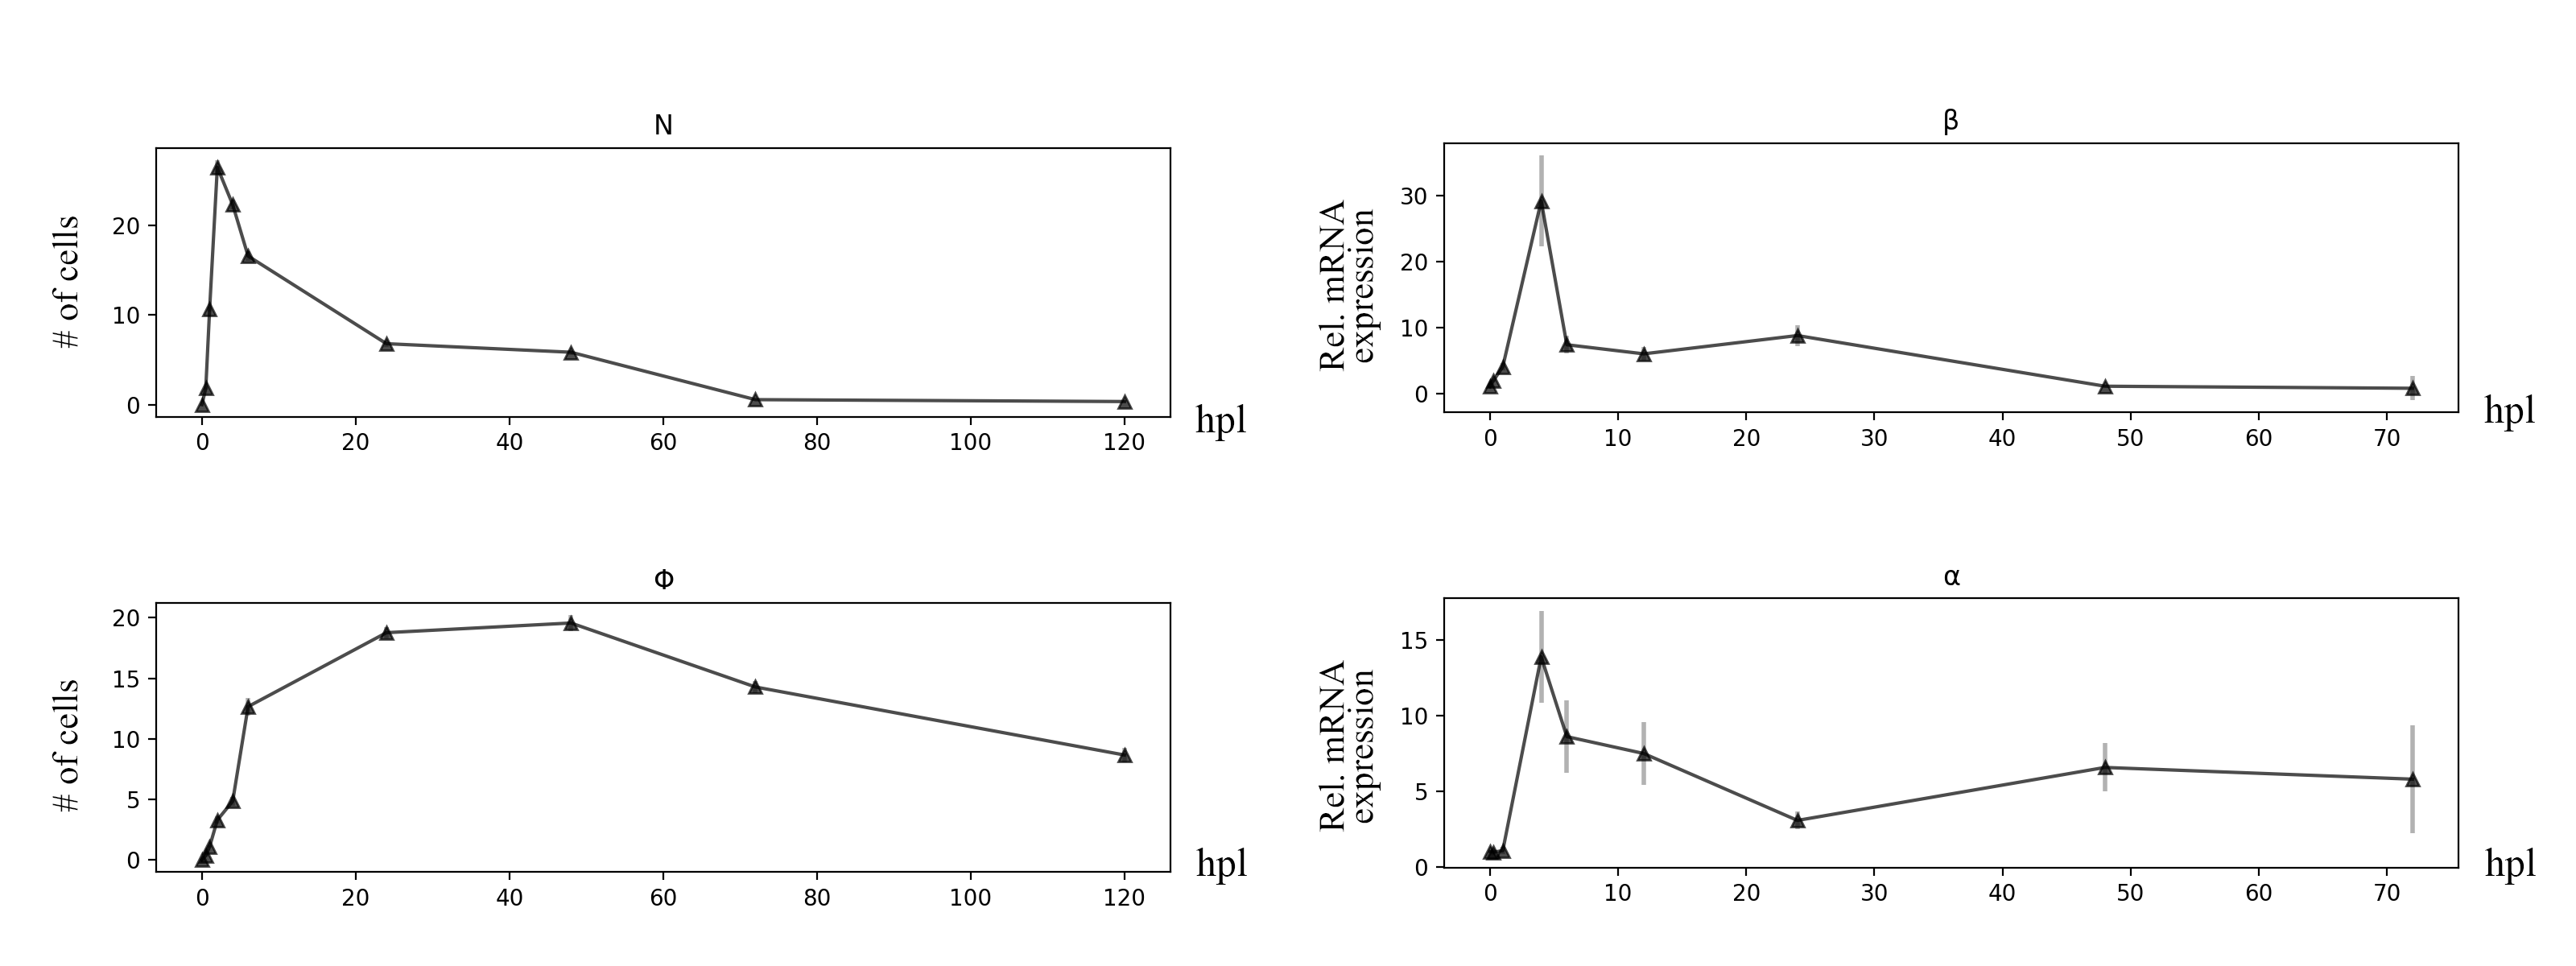
\includegraphics{fig/obs_curve.png}}
\end{center}

\caption[Mean of the observed data]%
{Mean of the observed data for neutrophil ($N$), macrophage ($\Phi$), il-1$\beta$ and tnf-$\alpha$, from experiment results of \cite{ref:Tsarouchas}. Error bars indicate standard error of mean} 
\label{fig:obs_data}

\end{figure}

\section{Hypothesis and Models}

5 models in total are proposed according to different hypothesis. At first our tests and implementations of ABC SMC for parameter estimations use only the basic model for developing propose. After the parameter estimation framework is built and tested, more models are proposed, in order to calibrate and adjust the basic model such that it can represent the observed regeneration process better or can be used to test our hypothesis. 

All these models assume the involved interactions is within two kinds of cells (neutrophil and macrophage) and two kinds of cytokines (il-1$\beta$ and tnf-$\alpha$) and use the data presented in Figure \ref{fig:obs_data} for the inference task. Interactions or effects from other cells or cytokines is not considered as there might not be corresponding data available.

\subsection{Basic model}

A preliminary model is proposed according to \cite{ref:Tsarouchas} and used to build and test the inference framework code. An interaction map of the model is shown in Figure \ref{fig:m1}. This model is a simplification a the process described in \cite{ref:Tsarouchas} with some minor interactions ignored. To describe the parameters' units, we denote the unit of $N$ and $\Phi$ i.e. number of cells as `cell', and denote the unit of $\beta$ and $\alpha$ i.e. relative mRNA expression as `unit' for simplicity.

\begin{figure}
    \begin{center}
    \resizebox{0.4\hsize}{!}{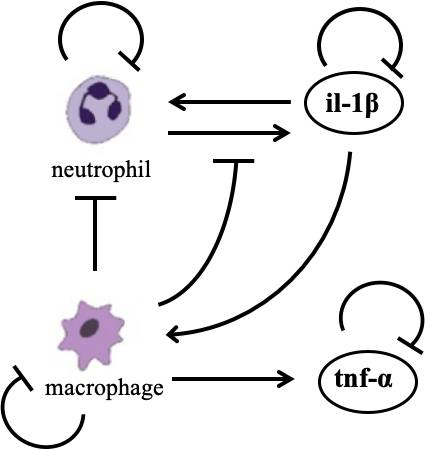
\includegraphics{fig/model1.png}}
    \end{center}
    
    \caption[Interactions modelled in the basic model]%
    {Interactions modelled in the basic model (model 1) based on Tsarouchas et al.\cite{ref:Tsarouchas}. Lines ended with arrow represent promoting effect, lines ended with T-connectors represent inhibition} 
    \label{fig:m1}
    
\end{figure}

It is assumed that there are negative feedbacks for all the variables. MORE DESCRIBE.

\begin{align}
    \label{eq:model1}
    \begin{split}
        &\frac{\mathrm{d} N}{\mathrm{d} t}=\lambda_N+\kappa_{N\beta}\beta-\mu_NN-\nu_{N\Phi}N\Phi\\
        &\frac{\mathrm{d} \Phi}{\mathrm{d} t}=\lambda_\Phi+\kappa_{\Phi\beta}\beta-\mu_\Phi\Phi\\
        &\frac{\mathrm{d} \beta}{\mathrm{d} t}=\frac{s_{\beta N}N}{1+i_{\beta\Phi}\Phi}-\mu_\beta\beta\\
        &\frac{\mathrm{d} \alpha}{\mathrm{d} t}=s_{\alpha\Phi}\Phi-\mu_\alpha\alpha
    \end{split}
\end{align}

\begin{table}[h!]
\centering
\begin{tabular}{|c c c|} 
 \hline
 Parameter & Definition & Units\\ [0.5ex] 
 \hline\hline
 $\lambda_N$ & Self-increase rate of neutrophil & $cell/h$  \\ 
 $\kappa_{N\beta}$ & Promoting effect coefficient by il-1$\beta$ & $cell/(unit\cdotp h)$\\
 $\mu_N$ & Coefficient of negative feedback of $N$ & $h^{-1}$ \\
 $\nu_{N\Phi}$ & Coefficient of inhibition of both $N$ and $\Phi$& $cell^{-1}\cdotp h^{-1}$ \\
 \hline
 $\lambda_\Phi$ & Self-increase rate of macrophage & $cell/h$ \\
 $\kappa_{\Phi\beta}$ & Promoting effect coefficient by il-1$\beta$ & $cell/(unit\cdotp h)$ \\
 $\mu_\Phi$ &  Coefficient of negative feedback of $\Phi$ & $h^{-1}$ \\
 \hline
 $s_{\beta N}$ & Production rate from $N$ & $unit/(cell\cdotp h)$ \\
 $i_{\beta\Phi}$ & Coefficient of inhibition to the production & $cell^{-1}$ \\
 $\mu_\beta$ & Coefficient of negative feedback of $\beta$ & $h^{-1}$ \\
 \hline
 $s_{\alpha\Phi}$ & Production rate from $\Phi$ & $unit/(cell\cdotp h)$ \\
 $\mu_\alpha$ & Coefficient of negative feedback of $\alpha$ & $h^{-1}$ \\
[1ex] 
 \hline
\end{tabular}
\caption{Parameters introduced in the basic model (model 1)}
\label{table:m1}
\end{table}

\subsection{Alternative models}

\paragraph{Model 2 and model 3}

As the observed data indicate, this dynamic system has a steady state where the  inflammation is resolved and immune cells should not be present at the injury site. Regarding this, the self-increase parameter $\lambda$ cannot be constant, thus a exponentially decaying $\lambda$ term is introduced and model 2 is proposed. (Eqn. \ref{eq:model2}). Also, the inhibition of il-1$\beta$ production, i.e. term $i_{\beta\Phi}\Phi$ is considered to be ignored for a more simple model, in which case the relative expression of il-1$\beta$ is only affected by the number of neutrophil and the negative feedback from itself. This case corresponds to model 3, written as Eqn. \ref{eq:model3}.

Model 2 and model 3 introduce one extra parameter $a$, which is a coefficient in the exponentially decaying $\lambda$, determining the decay speed, with the unit $h^{-1}$.

\begin{align}
    \label{eq:model2}
    \begin{split}
        &\frac{\mathrm{d} N}{\mathrm{d} t}=\lambda_Ne^{-at}+\kappa_{N\beta}\beta-\mu_NN-\nu_{N\Phi}N\Phi\\
        &\frac{\mathrm{d} \Phi}{\mathrm{d} t}=\kappa_{\Phi\beta}\beta-\mu_\Phi\Phi\\
        &\frac{\mathrm{d} \beta}{\mathrm{d} t}=\frac{s_{\beta N}N}{1+i_{\beta\Phi}\Phi}-\mu_\beta\beta\\
        &\frac{\mathrm{d} \alpha}{\mathrm{d} t}=s_{\alpha\Phi}\Phi-\mu_\alpha\alpha
    \end{split}
\end{align}

\begin{align}
    \label{eq:model3}
    \begin{split}
        &\frac{\mathrm{d} N}{\mathrm{d} t}=\lambda_Ne^{-at}+\kappa_{N\beta}\beta-\mu_NN-\nu_{N\Phi}N\Phi\\
        &\frac{\mathrm{d} \Phi}{\mathrm{d} t}=\kappa_{\Phi\beta}\beta-\mu_\Phi\Phi\\
        &\frac{\mathrm{d} \beta}{\mathrm{d} t}=s_{\beta N}N-\mu_\beta\beta\\
        &\frac{\mathrm{d} \alpha}{\mathrm{d} t}=s_{\alpha\Phi}\Phi-\mu_\alpha\alpha
    \end{split}
\end{align}

Model 3 can be regarded as a simplification of model 2, as it can be treated as model 2 with parameter $i_{\beta\Phi}=0$. Among the proposed three models, model 1 is a naive one that was proposed at very first time and used as an ODE `template' to build and test parameter inference framework. As the implementation was successful, model 2 and 3 was proposed as we were trying to calibrate some terms and find a better model. After fitting, model 2 is supposed to be better than model 1 as it corrects the problem that appears at the final time points (which relate to the steady state). Model 3 makes a small simplification on model 2 and is theoretically less `general' than model 2.

\paragraph{Model 4 and model 5}

After the first model selection experiment, it was found that some significant features presented in the observed data were not recovered by any of the existing model. To resolve this, attempts were tried to introduce more interactions within the dynamic system considering the biological and  mathematical context. Extra promoting effect to the expression of tnf-$\alpha$ was considered, by either adding a phenomenological term (which means the same effect as directly promoting but the underlying mechanism is unclean) or adding a term that represents a promoting effect to the production process of tnf-$\alpha$, namely model 4 (Eqn. \ref{eq:model4}) and model 5 (Eqn. \ref{eq:model5}).

\begin{align}
    \label{eq:model4}
    \begin{split}
        &\frac{\mathrm{d} N}{\mathrm{d} t}=\lambda_Ne^{-at}+\kappa_{N\beta}\beta-\mu_NN-\nu_{N\Phi}N\Phi\\
        &\frac{\mathrm{d} \Phi}{\mathrm{d} t}=\kappa_{\Phi\beta}\beta-\mu_\Phi\Phi\\
        &\frac{\mathrm{d} \beta}{\mathrm{d} t}=s_{\beta N}N-\mu_\beta\beta\\
        &\frac{\mathrm{d} \alpha}{\mathrm{d} t}=s_{\alpha\Phi}\Phi-\mu_\alpha\alpha+d_{\beta\alpha}\beta
    \end{split}
\end{align}

\begin{align}
    \label{eq:model5}
    \begin{split}
        &\frac{\mathrm{d} N}{\mathrm{d} t}=\lambda_Ne^{-at}+\kappa_{N\beta}\beta-\mu_NN-\nu_{N\Phi}N\Phi\\
        &\frac{\mathrm{d} \Phi}{\mathrm{d} t}=\kappa_{\Phi\beta}\beta-\mu_\Phi\Phi\\
        &\frac{\mathrm{d} \beta}{\mathrm{d} t}=s_{\beta N}N-\mu_\beta\beta\\
        &\frac{\mathrm{d} \alpha}{\mathrm{d} t}=(s_{\alpha\Phi}+f_{\beta\alpha}\beta)\Phi-\mu_\alpha\alpha
    \end{split}
\end{align}

\begin{table}[h!]
    \centering
    \begin{tabular}{|c c c|} 
     \hline
     Parameter & Definition & Units\\ [0.5ex] 
     \hline\hline
     $d_{\beta\alpha}$ & Coefficient of promoting effect from $\beta$ & $h^{-1}$  \\ 
     \hline
     $f_{\beta\alpha}$ & Coefficient of promoting the production of $\alpha$ by $\beta$ & $cell^{-1}\cdotp h^{-1}$  \\ 
     \hline
    \end{tabular}
    \caption{Parameters introduced in model 4 and 5}
    \label{table:m45}
\end{table}



\subsection{Model evaluation and comparison}

[general topics on evaluating a model]

[bayes factor for model selection]

\subsection{Limitations}

[hypothesis]

[available data]

[model misspecification]

% \begin{figure}

% \begin{center}
% \resizebox{0.30\hsize}{!}{
\includegraphics{logos/crest_bw}}
% \end{center}

% \caption{The University Crest}
% \label{fig:eucrest}

% \end{figure}


% see the man page for dvips for details of the special command which is
% much more powerful than is shown here. It allows offsets in the
% horizontal and vertical and scaling in x and y.

% choosing suitable values for offset and scale can be a tiring matter
% of trial and error.

% note that labels do not need to include a description of the object
% they are labelling but it can be helpful, eg \label{fig:figurename}.

% You can use a label on a figure to refer to it later. The university
% crest is in \ref{fig:eucrest}. Note that you should not use phrases like
% ``the figure above'' or ``the following figure'' since Latex may move
% the figure relative to the text if it cannot be fitted onto the current page.









\chapter{Parameter estimation and model comparison}

Estimation of  parameters in the proposed models is the main task of this section, which involves the implementation of ABC SMC and several experiments. ABC SMC-based model selection is another task that can be easily conducted with the developed parameter inference framework.

The build and test of code were under \verb|Python| environment with \verb|pyABC|\cite{ref:pyabc}. Some other code e.g. shell script and \verb|R| code are also used to perform the experiments and analyse the results. Software and system environment used in our implementation can be found at Appendix A. The build and test were performed on local computers and HPC facilities available within EPCC.






\section{Implementations and code}

[ABC implementations details, e.g. distance, population, ODE related functions]

[how the code is developed and built]

According to our preliminary studies, ABC SMC framework implemented using \verb|pyABC| in \verb|Python| was adopted in this project. \verb|pyABC| is a popular SMC software packages \cite{ref:pyabc} that has been used form many SMC studies and applications \cite{ref:adpt_pop}. \verb|pyABC| provides an open-source framework for likelihood-free inference, which is an implementation of ABC SMC algorithm and a tool-box for our own inference and analysis tasks. Besides, it supports multi-core execution implemented using \verb|multiprocessing| package for scaling-up, which is of our interests and suitable for the followed performance experiments.

The inference framework code for the project was developed and tested in local environment (macOS 10.15.6, see Table \ref{table:local_macine}) at first, then the functional version was deployed on compute node of ARCHER and Cirrus for parameter inference experiments and model selection task. The scaling-up experiment was performed on Cirrus, and the profiling and its analysis were performed on local machine. Some development and debug were on the remote machines to ensure experiments run correctly on compute node.

The ODE model-related code and utilities were firstly developed to enable reusable functions, variables and data calls. It includes the code for the ODE models, ODE solver, data structures, data format transform functions etc. By doing this in a separate code file, we can change options and activate ABC SMC easily in the implementation code file, without creating definition and duplicated code for the models and parameter priors.

Some modifications were made to the source code of \verb|pyABC|. For example, the laboratorial measured data were not considered `complete' for modeling and analysis purpose: the available time points for cells and cytokines are different, e.g. cell number was not measured at 0.25 hpl and cytokines' expression was not measured at time point 120 hpl. These missing values were treated as `ignored' when calculating the distance between observed data and simulated data. To cope with this built-in distance function code is modified.

Analysis code was also wrapped up into functions which can be easily called after an ABC SMC run is finished, which includes multiple visualisations and summary statistic of the results. For different tasks there are also separated analysis code file. Other analysis tools used in the project include built-in database visualisation tool, R code and Microsoft Excel.

The project code was managed via \verb|git| version-control and available as a GitHub repository\footnote{\url{https://github.com/chaolinhan/MSc_Project}}; it also made the cross-hardware synchronisation of code versions convenient.

After several development iterations, code files for ABC SMC implementation now mainly had two types: code files for infer-back experiments (udsing synthetic data), and code files for parameter inference (using experimental data). Model selection can be easily done by adding more model to the implementation code file.


% \section{Parameter estimation}

% [implementation details and options/ settings that are affecting the ABC]







\section{ABC SMC and model hyperparameters experiments}

As the key focus of this project is on the parameter estimations of dynamical system, the ability of inference on the proposed models was firstly examined before actual inference using the experimental observed data.

In the first part, synthetic data is used with known true parameter values. The algorithm implementation is evaluated by the efficiency and goodness of resultant model under different implementation options and ABC SMC hyperparameters.

Then according to findings in the first part, several options with good performance are tried in the inference using experimental observed data (Figure \ref{fig:obs_data}). To obtain a more accurate and general results, these experiments are repeated for 3 or more times.

[including the options that are tested/ tried/ not adopted]

[including experiments results and discussions]

[how do these options correspond to biological model and how to set them accordingly for proposed model]

The ABC SMC inference can have largely different performance when using different hyperparameters and implementation options. To firstly test the ability of inference and observe the results of different options, synthetic data with known true parameter values are used as target data. The true value of parameters that are used to generate synthetic data is listed in Appendix B.1. These true values are firstly obtained by fitting a least square fit of model 1 onto the experimental data (Figure \ref{fig:infer_back_data}), the target data is then generated using these parameter values via ODE solver in \verb|Python|. 

\begin{figure}[h!]
    \begin{center}
    \resizebox{1.0\hsize}{!}{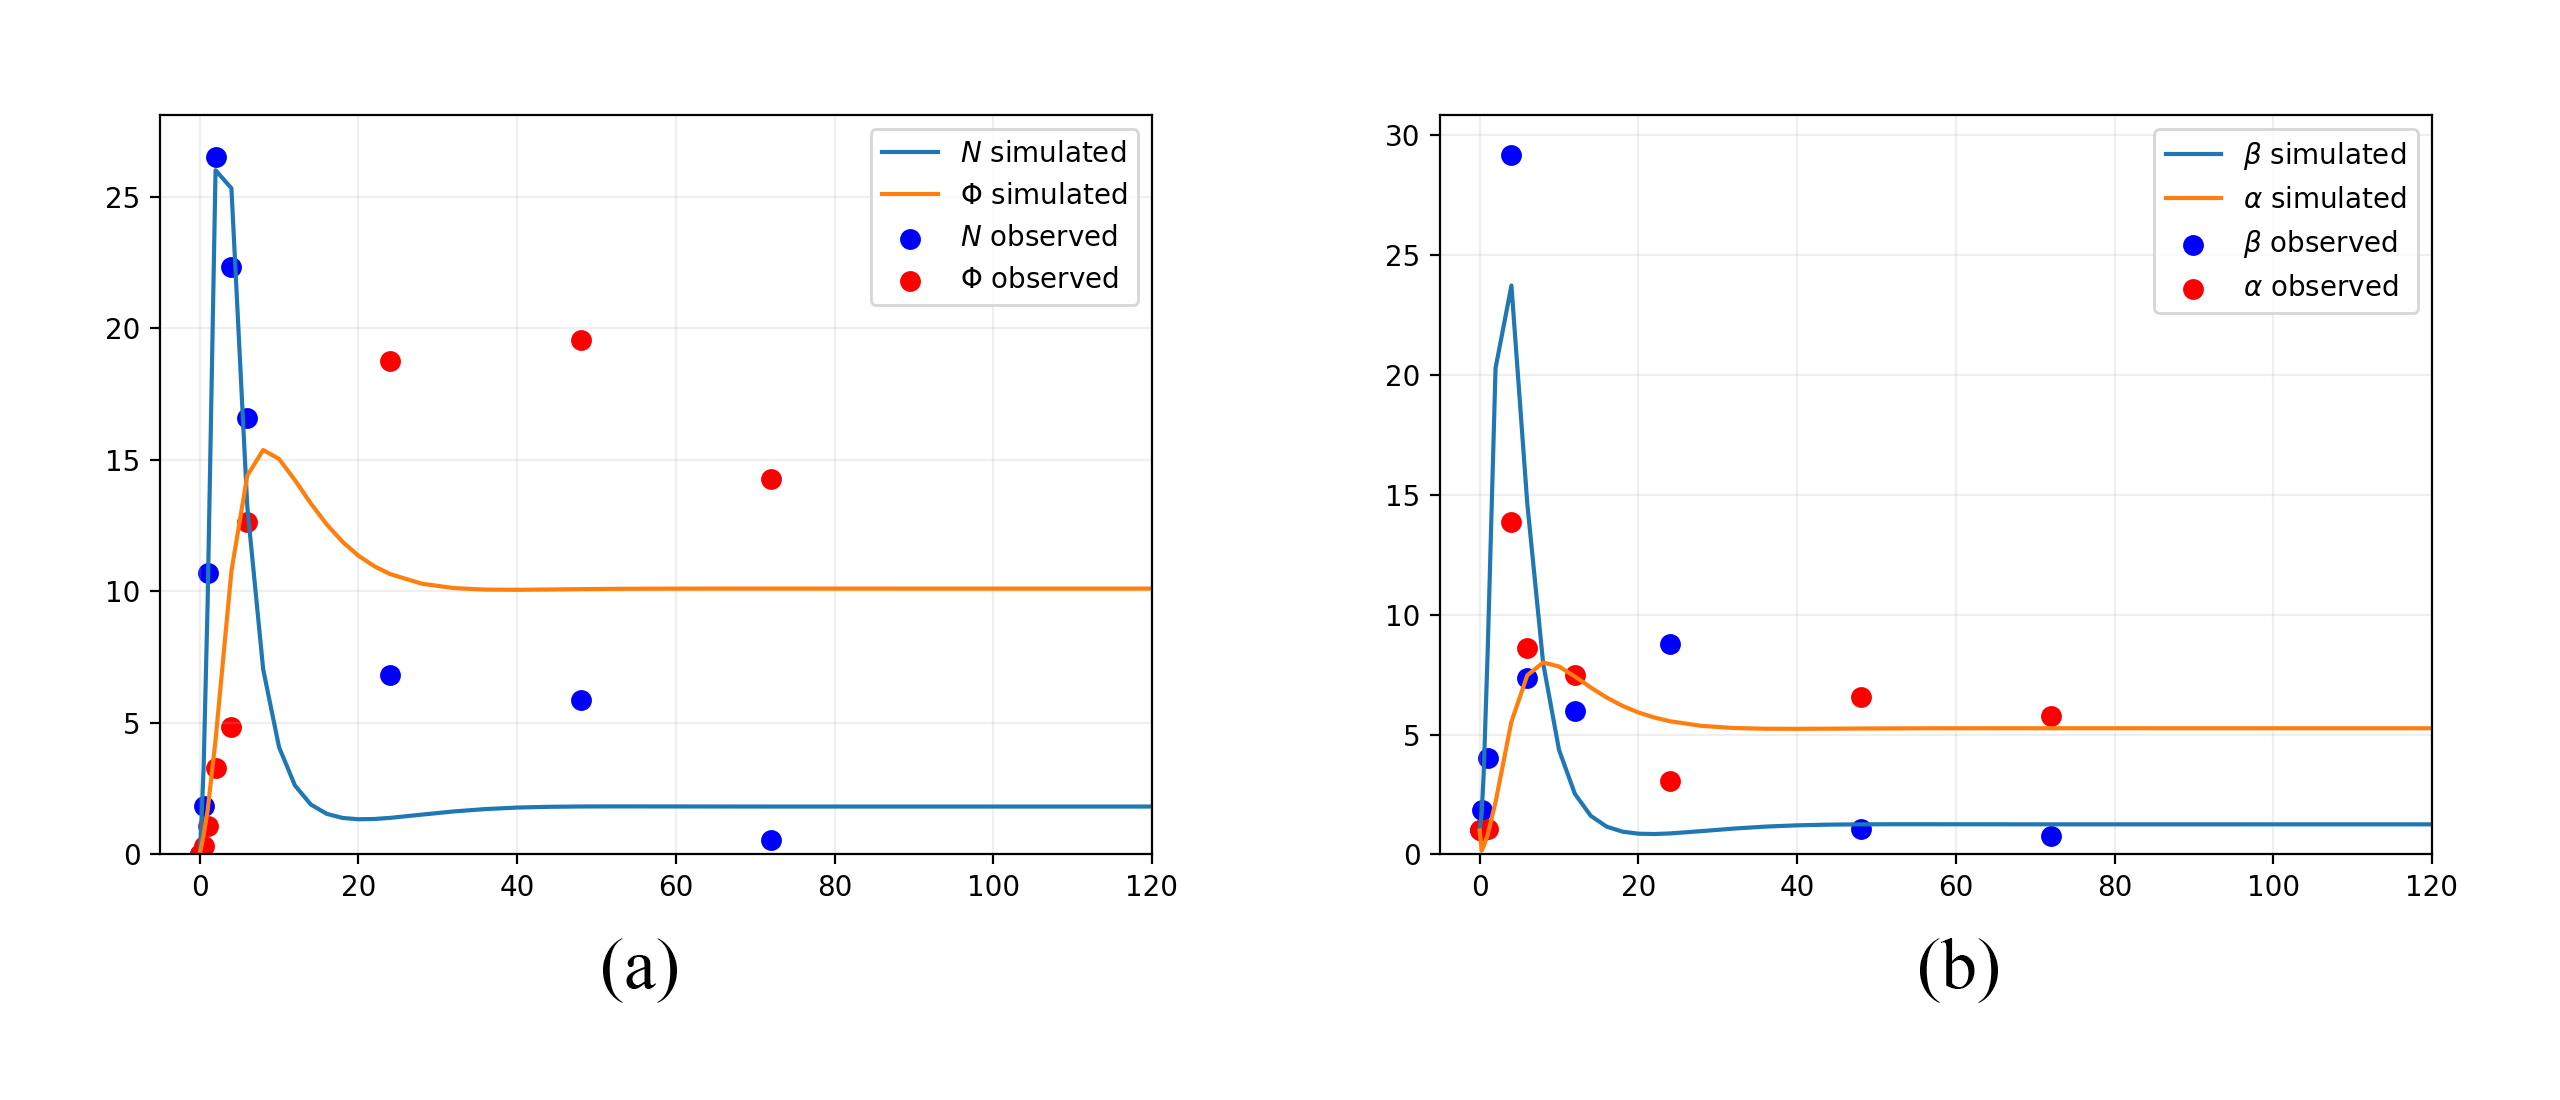
\includegraphics{fig/LS.png}}
    \end{center}
    
    \caption[Synthetic data generated with known parameter values]%
    {Synthetic data generated with known parameter values (line plot), compared to experimental data (scatter plot). Known parameter values are obtained from a least square fitting of the observed data} 
    \label{fig:infer_back_data}
    
\end{figure}

[TABLE for known parameter values]

[why use synthetic data]

Among them the following topics are studied using the synthetic data.

\subsection{Perturbation kernels}

Perturbation kernels work in the sampling process. In each generation $t$, samples are firstly taken from the previous population $\{\theta_{t-1}\}$ with weights $\{w_{t-1}\}$, then perturbed using the perturbation kernel $K(\theta|\theta^*)$. We keep sampling until $N$ particles are accepted, where $N$ is the pre-set population size. After that the new weights are calculated and normalised. 

\begin{figure}[t!]
    \begin{center}
    \resizebox{1.0\hsize}{!}{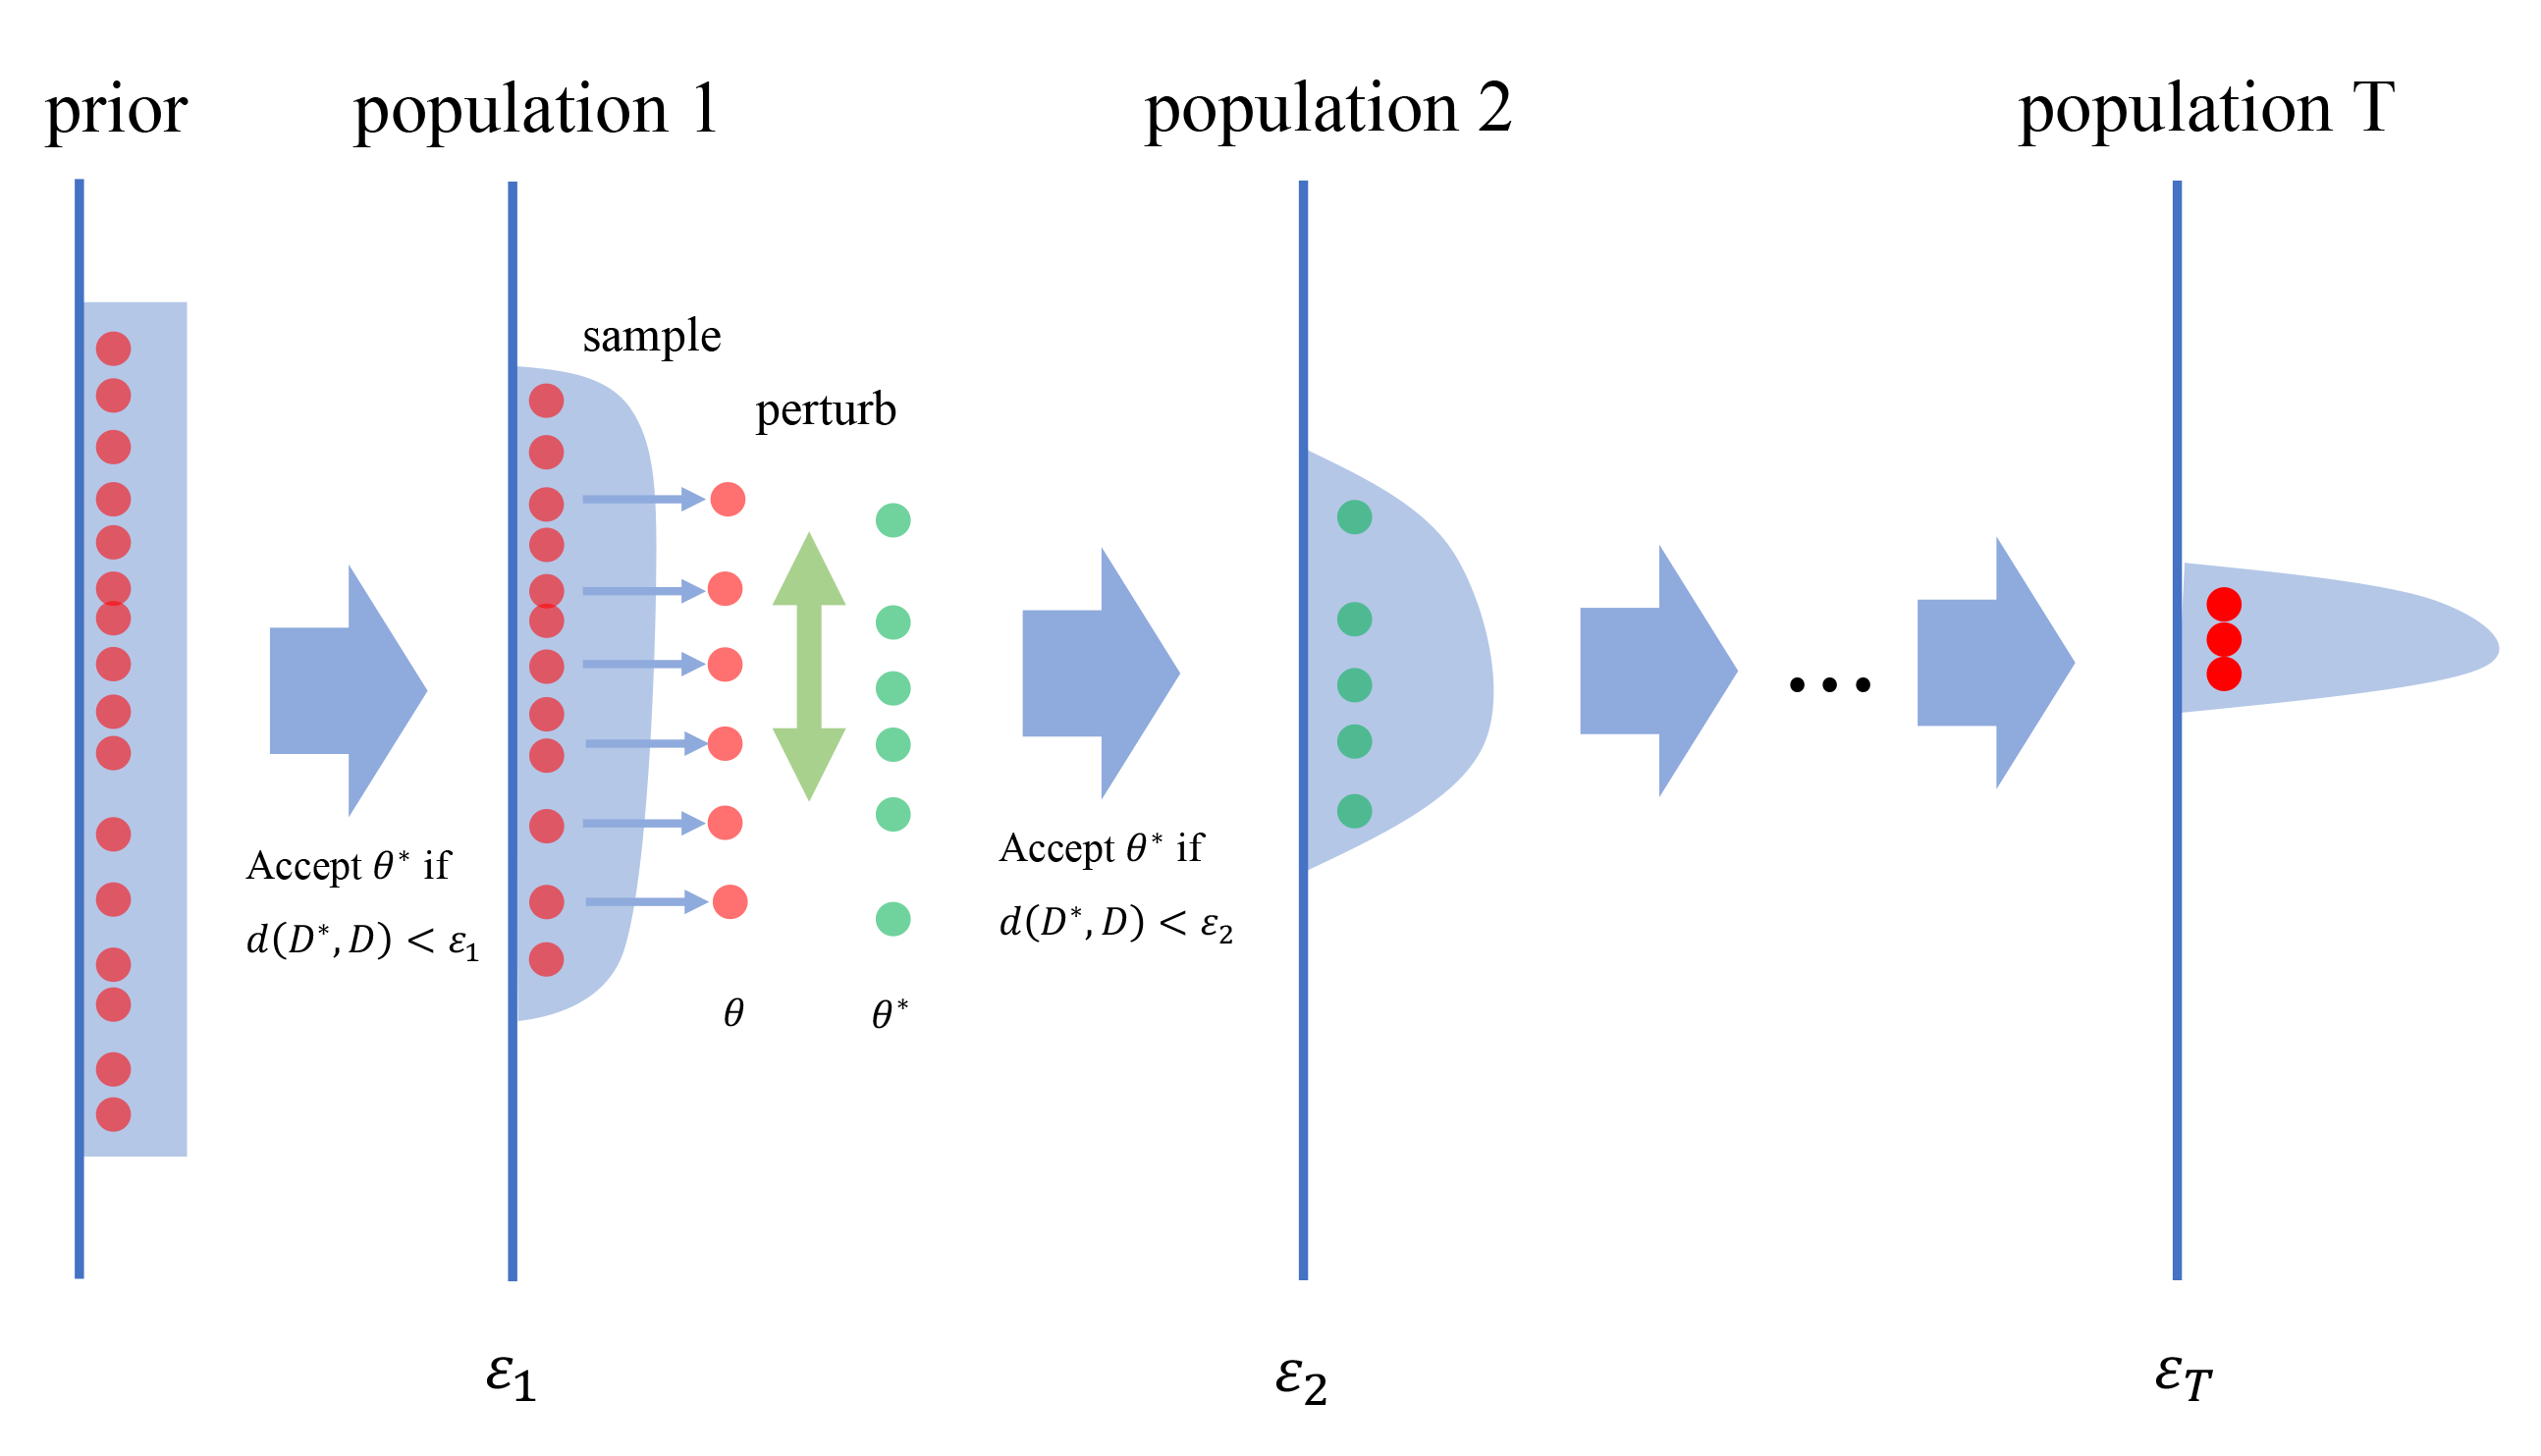
\includegraphics{fig/smc.png}}
    \end{center}
    
    \caption[ABC SMC sampling process]%
    {ABC SMC sampling process. $\theta^*$ denotes a sample drawn from previous population, which is used to generate simulated data $D^*$. $d$ is a distance measurement, $d(D^*,D)$ represents the discrepancy between observed data and simulated data. for each population $t$, $\epsilon_t$ is a threshold criterion to determine whether to accept that drawn sample} 
    \label{fig:smc}
    
\end{figure}

The perturbation kernel is called in the sampling of every particles and determines how the new perturbed particle is chosen, thus it is influential to both computation complexity and the resultant posterior distribution. Generally, a local perturbation kernel may face the risk of being stuck in local modes (e,g., local optimal), but it may need less computational operations, or could generate a population with a higher acceptance rate if the successive epsilon values are close; A kernel with wide variance, or spreading out in a large space could help in resolving the local optimal problem by a more thoroughly exploration of the parameter space, however it can be more computation-intensive and result in a lower acceptance rate. A desired optimal kernel should balance the trade-offs; their property and criteria is discussed in \cite{ref:kernel}.

There are several common choice of perturbation kernels. Among them multivariate normal kernel and local M-nearest neighbour model is preferred to be applied on our models. A covariance matrix $\Sigma_t$ of accepted particles is calculated form previous generation and used in multivariate normal kernel: $K(\theta|\theta_{t-1})\sim\mathcal{N}(\theta_{t-1}, \Sigma_t)$. It is illustrated to be more efficient than uniform kernel and component-wise normal kernel in relecting the true posterior structure \cite{ref:kernel}. It has been proved to perform well in several dynamic system models \cite{ref:abcsysbio, ref:compare, ref:disease} for the parameter estimation and model selection tasks. The $scaling\in(0,1]$ parameter in \verb|pyABC| will be multiplied to the covariance to produce a `narrower distributed' perturbation result.

Local M-NN kernel provided by \verb|pyABC| is also tried to provide a comparison. A local kernel density estimation (KDE) fit is used with M nearest neighbours considered.

The kernel experiments is designed to explore the efficiency of SMC on our dynamical systems. Given the same fixed threshold schedule, kernels that need less total samples and have higher acceptance rate would be our preference. The experiments compared multivariate normal kernel with local MNN kernels with different parameters, using synthetic data to infer back the parameters. The acceptance rate among each time point and total required samples are compared after the experiment to give suggestions on the kernel selection in the real data inference. As the threshold schedule is fixed, the final population should have similar discrepancy to the target data thus here the goodness of fit i.e. recover of target data trends/features and errors of the inferred parameters compared to true values is not discussed.

\subsubsection{Kernel experiment results}

To compare kernels, a fixed schedule schedule is used with minimal epsilon i.e. $\epsilon_t$ set to 10.0. From the total required samples graph Figure \ref{fig:kernel1}, the efficiency can be compared. Among the tested kernels, the local M-NN with M=50 has the best performance: it requires the least number of samples and 
has higher acceptance rates among almost all generations. Local M-NN with M=750 is the slowest kernel.

For local M-NN kernels, generally a greater M will lead to lower acceptance rate and 
more required particles in each generation. As shown in Figure \ref{fig:acceptance1}, local M-NN with M=750 is the lowest curve. Consequently, if greater M is test, then it will have even lower acceptance rates; the maximum M=2000 (whole population is considered) will have the lowest acceptance rates.

\begin{figure}
    \begin{center}
    \resizebox{1.0\hsize}{!}{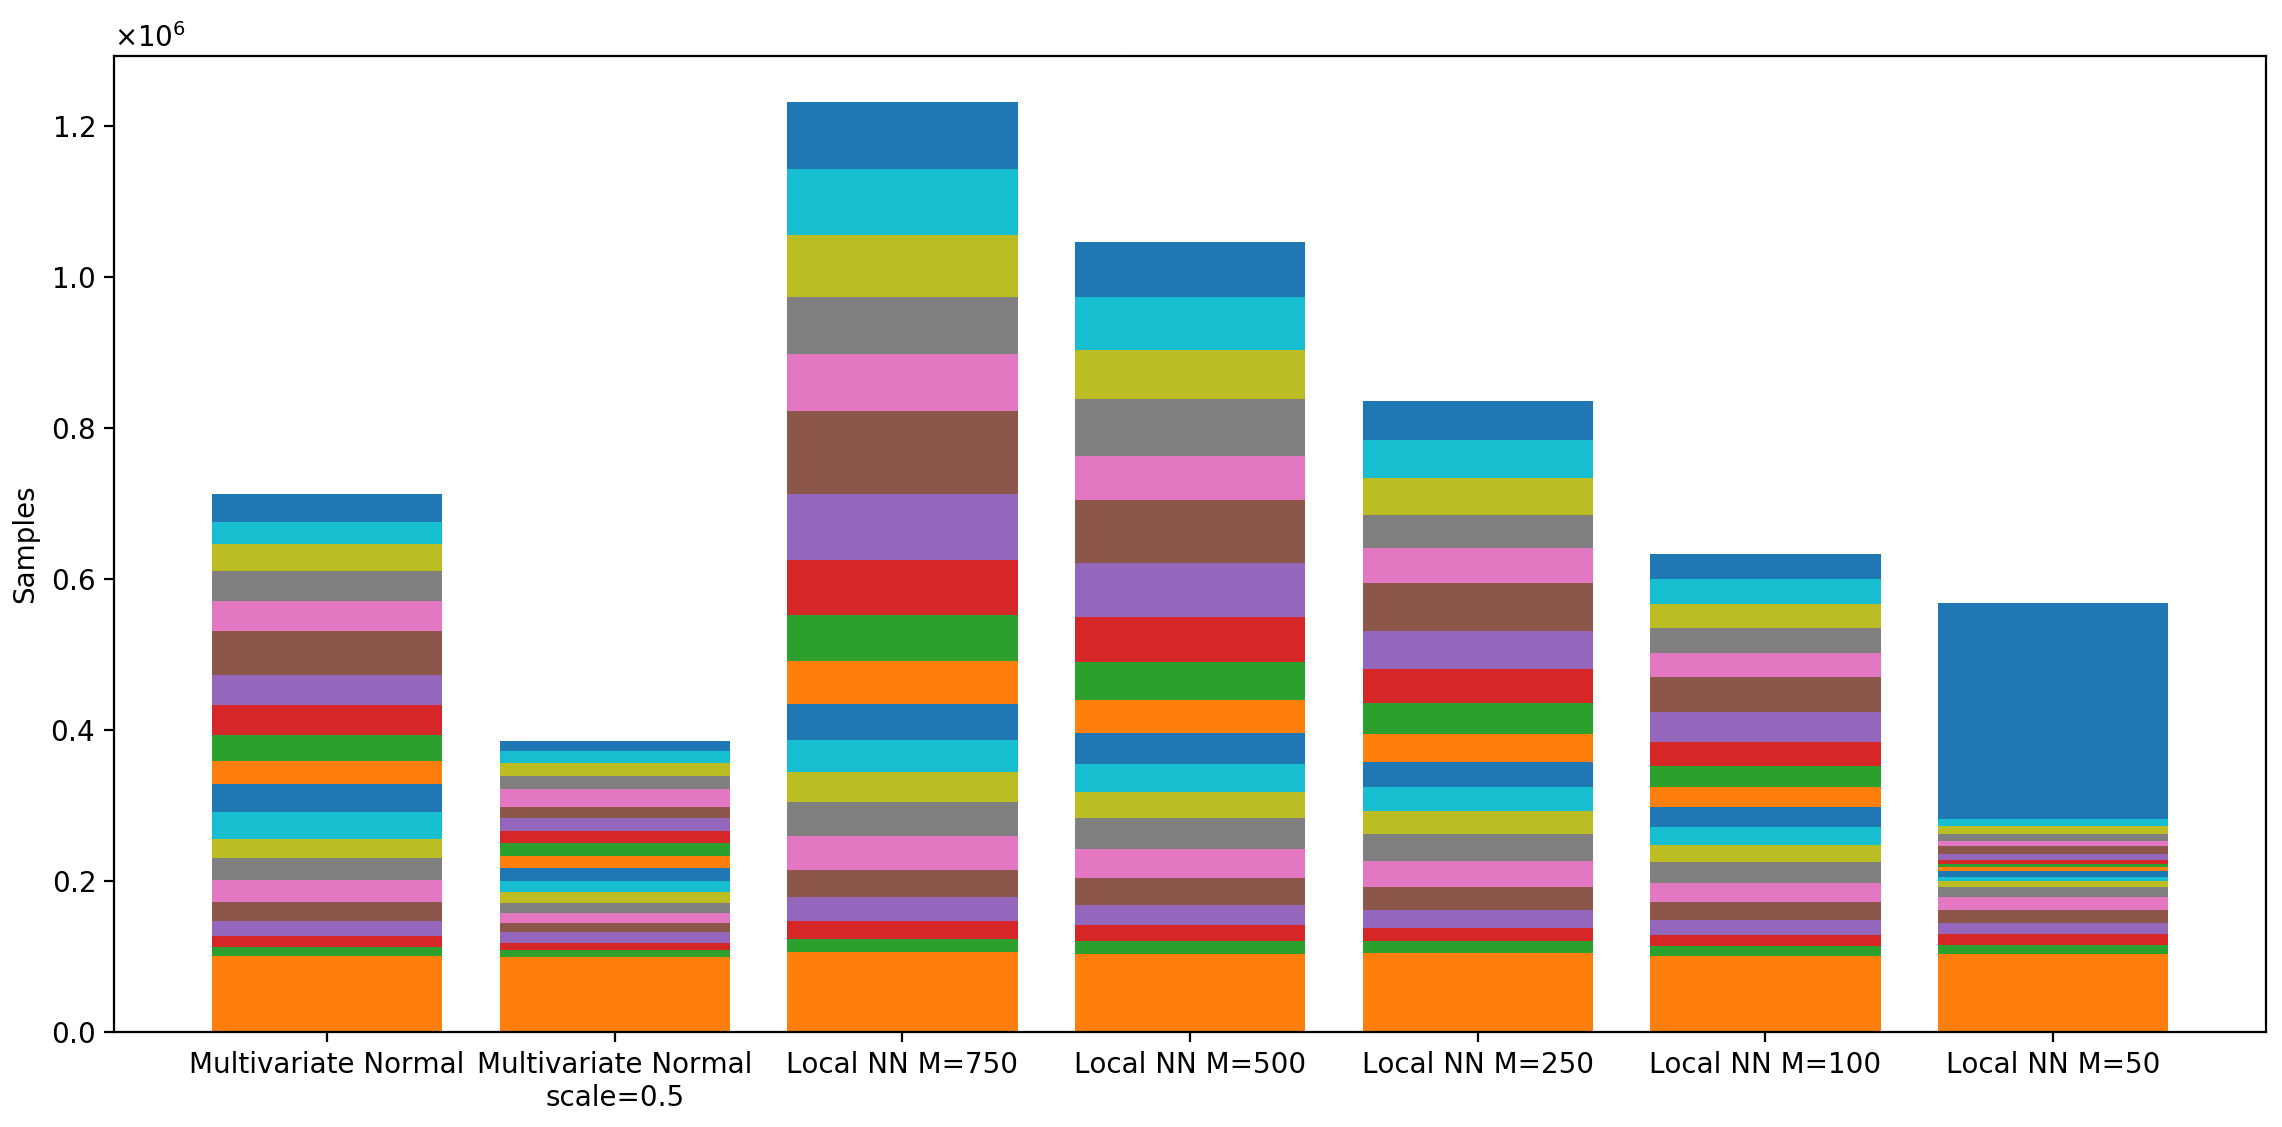
\includegraphics{fig/kernel1.png}}
    \end{center}
    
    \caption[Total required samples of different kernels]%
        {Total required samples of different kernels after 20 populations (2000 particles in each population). Different color represents different generations (bottom to top: population 1 to population 20)}
    \label{fig:kernel1}

    \vspace*{\floatsep}

    \begin{center}
    \resizebox{1.0\hsize}{!}{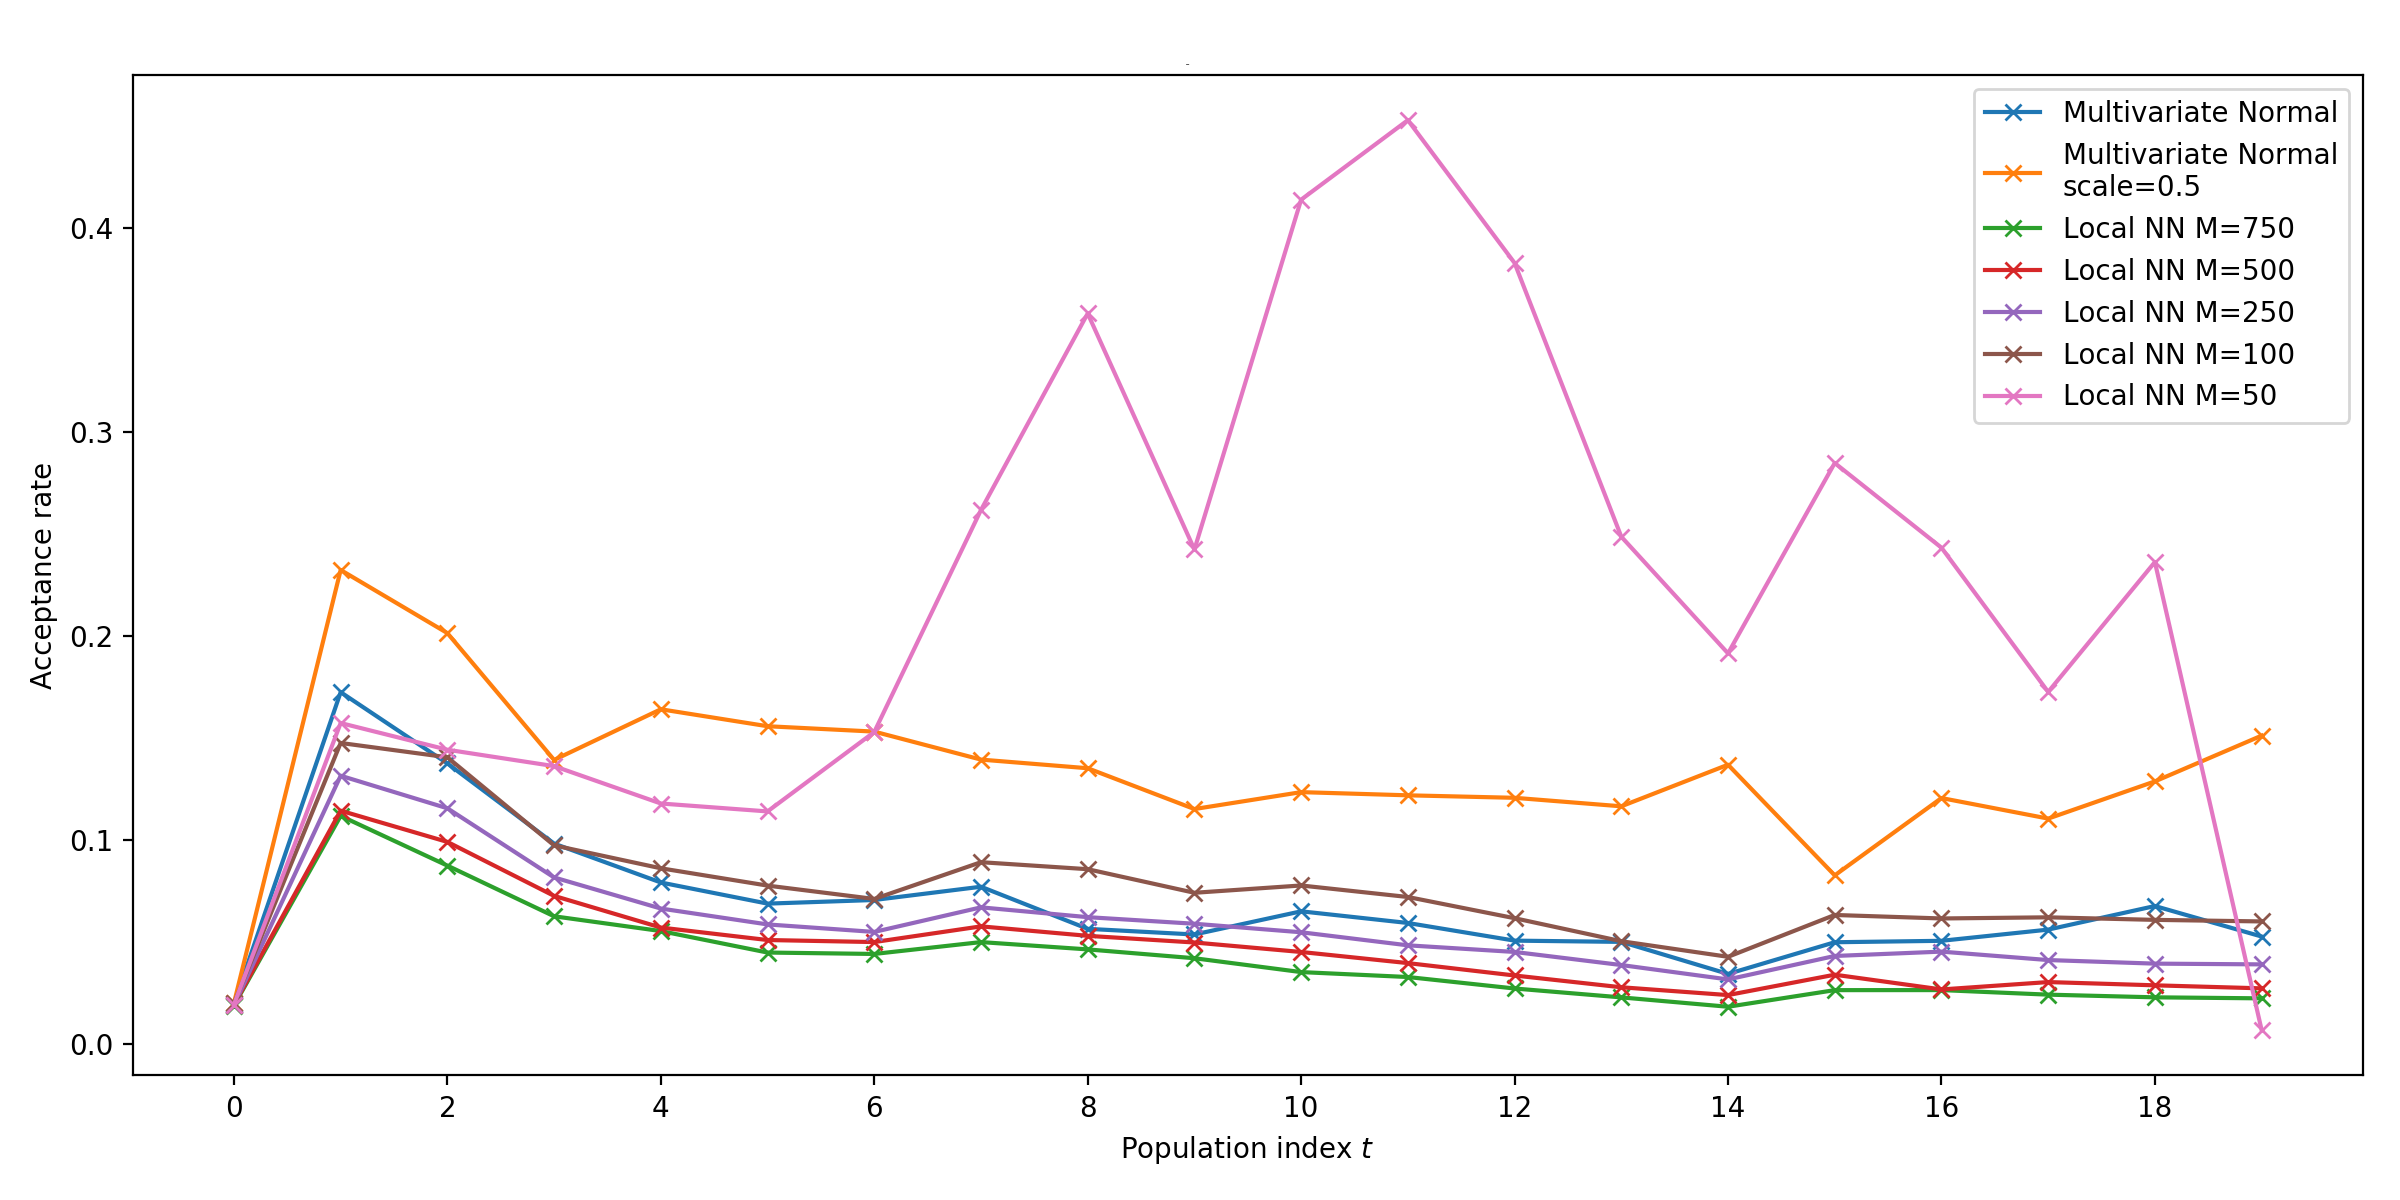
\includegraphics{fig/acceptance1.png}}
    \end{center}
    
    \caption[Acceptance rates of different kernels]%
    {Acceptance rates of different kernels in 20 populations. Each population has 2000 particles}
    \label{fig:acceptance1}
    
\end{figure}

Multivariate normal kernel has a performance between local M-NN M=250 and M=100. It proves that rather than a trivial normal kernel, multivariate normal kernels is more efficient facing the concentrations of joint distributions among multiple parameters \cite{ref:kernel}. `Scaling' option can narrower the distribution calculated from the last population, thus making the kernel more `local' by sampling under a smaller variance. Similar to small M in local M-NN, small `scaling' is also more efficient in our experiment of the model 1. Besides the fixed threshold schedule, a median threshold schedule with the same final threshold $\epsilon_{20}=10.0$ is also tested and similar results are observed (Figure \ref{fig:kernel2} and \ref{fig:acceptance2}, Appendix B2).

It seems that a more `local' kernel can give better performance by efficiently sampling around concentrations in parameters' distribution and approximate the posterior distribution. This holds in most cases under a given target final threshold value $\epsilon_t$, however may not produce the proper result want: a more local kernel, e.g. local M-NN with small M and multivariate normal with `scaling' is more likely to be stuck in local optimality, as the kernel is less likely to sample particles that are far from local concentrations, although these local optimal are still accepted under given threshold. In other words, using local kernels the epsilon may quickly converge to to local optimal; if a even smaller epsilon is desired, the local kernel can hardly generate enough particles to find another matched local modes. Also, the shapes of posterior distribution will affect the performance of local kernels \cite{ref:kernel}. One obvious example is presented in Figure \ref{fig:kernel1}, where local M-NN with M=50 suffered from a local optimal: the last generation takes much more samples to meet the required threshold.

\subsubsection{Conclusion} Local kernels can be fast bur unstable in some case; for a general parameter inference of our models, multivariate kernels are preferred, as a good fit is our prior target; some local kernels are also worth trying after the multivariate normal kernel, e.g. local M-NN with M$\leq 250$ (for population size of 2000, i.e. 12.5\% of the population) and multivariate normal with scaling. Also multivariate M-NN is worth trying, although it is not built in \verb|pyABC| and requires additional implementations.


% \begin{figure}
%     \begin{center}
%     \resizebox{1.0\hsize}{!}{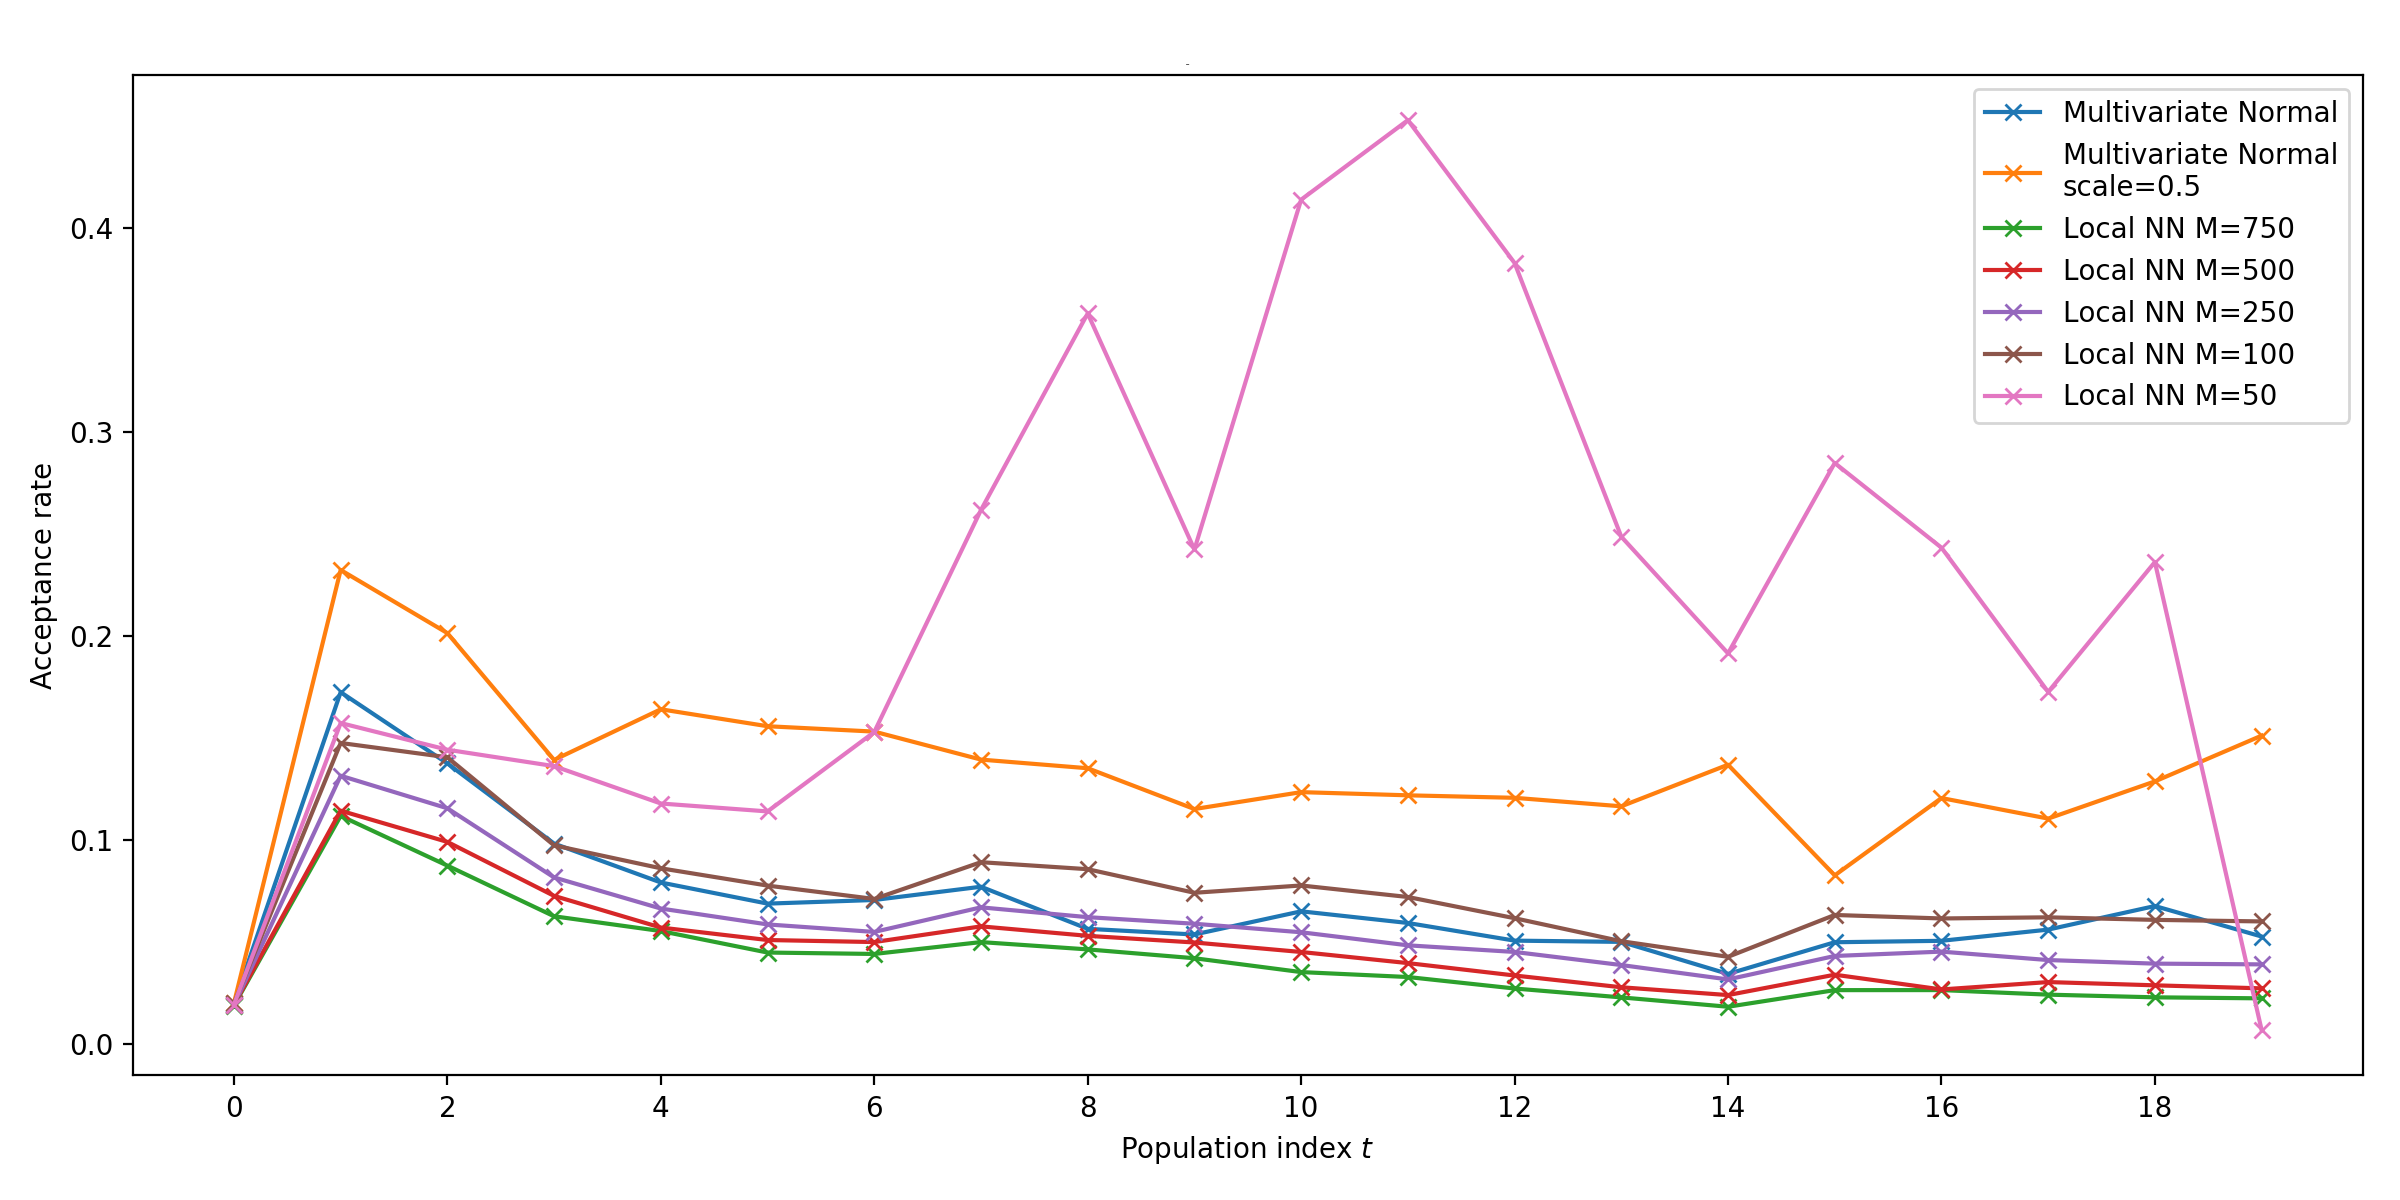
\includegraphics{fig/acceptance1.png}}
%     \end{center}
    
%     \caption{Acceptance rates of different kernels}
%     \label{fig:acceptance1}
    
% \end{figure}


\subsection{Adaptive functions and factors}

[how adaptive distance work]

SMC can be more adaptive by introducing adaptive distance function and adaptive population; besides, factors can be applied to manually `normalise' the data.

The trivial distance function is set to Euclidean distance (2-norm distance)

\begin{align}
    \label{eq:dis}
    D=\sqrt{\sum_i \Delta x_i^2}
\end{align}

where $i$ is the index of data points and $\Delta x_i$ is the discrepancy between  observed data and simulated data at data point $i$, i.e. $\Delta x_i = x_{i, simulated}-x_{i, observed}$. In this case data points are 12 time points of four variables i.e. 48 data points in total.

A weighted 2-norm distance can be written as 

\begin{align}
    \label{dis_w}
    D=\sqrt{\sum_i w_i \Delta x_i^2}
\end{align}

where a weight $w_i$ is assigned to every data point. If data point $i$ have a higher weight, then the data value is regeared to be more informative, i.e. giving more help in inferring the true posteriors; weights can be either pre-set according to prior knowledge of the problem, or using adaptive method to be dynamically calculated according to , known as adaptive distance. 

Adaptive distance is changing the weights of all data points after each generation iteration, trying to assign informative data points higher weights. Additionally, implementation of adaptive in \verb|pyABC| also introduces additional factors $f_i$ multiplied to weights \cite{ref:adpt_dis} 

\begin{align}
    \label{dis_f}
    D=\sqrt{\sum_i f_iw_i \Delta x_i^2}
\end{align}

Factor is helpful as an option for efficiency. When some data points are equally informative, the manually pre-defined can make the distance more focused on certain data point, or behave like a normalisation that can balance the scales of different summarised statistics (here is the 48 mean values). There are two appliance case studied: (1) factors used as an normalisation option and (2) factors used to give more focus on some features of the observed data. For (2), as we noticed that the main features (e.g. rapid increase, peaks, fluctuations) are mostly observed in the first half of the time points i.e. 0 - 30 hpl, factors are tried in the later parameter estimation of real data where a more accurate fit of the curve is desired.

Adaptive population \cite{ref:adpt_pop} can adapt the population size of each generation according to the mean correlation of variation error of the previous population. In our early test the maximal population size that is allowed is set to 5,000 and the adaptive strategy always select the upper bound, as a results of wide parameter space or the wide posterior approximation shape.

[what is factor]

[what is adaptive distance]

\subsubsection{Experiments results}

[FIGURE here]

Two types of factors and adaptive distance function are tested by running the same number of generations (20 generation, 2000 particles per generation). From FIGURE, by applying factors the total required samples are less, and the adaptive distance requires much less samples; their acceptance rates are also higher than the standard one. It seems that adaptive function and factors could help to converge more quickly.

However considering the result after 20 generation (FIGURE), the resultant model gives the contrary preference. Applying factors and using adaptive distance can lead the resultant model less accurate (after the same generation iterations): they have wider inter-quantile range and may requires more generations to converge.


\subsubsection{Conclusion} We noticed the significant efficiency improvement of these adaptive options; they can largely improve the acceptance rate in some cases. However, as the factors and weights are directly multiplied to $\Delta x$ and thus the metrics for distance are changed, a direct compare of the efficiency under the same threshold schedule is unfeasible; after the same number of generations they can reach a small $\epsilon_t$ but still the approximated posterior is not as accurate as the standard implementation. AS a result, our implementation of the parameter inference will only consider standard distance function and factors are only tested for improvements (FIGURE).


\subsection{Data size, prior distribution and population}

[experiments plan]

Some other hyperparameters, e.g. feed-in data size, prior distribution, number of populations and number of particles in each population were also of our interest. Experiments were designed to explore how these options affect the goodness of fit and efficiency of the implementation.

Regarding the dynamic systems model, SMC was applied with two data size options, three prior distribution (uniform distribution, wider uniform distribution and log-uniform distribution). The population options i.e. population size and number of populations were also tried with different values. These experiments intended to give suggestions on the later SMC implementation on experimental data.

\subsubsection{Experiments results}

The results from data size and prior distribution range is shown in FIGURE. The standard implementation is fed with 120 data points (30 data points for each of the four variables), the `less data' is fed with 48 data points, which is the case of the real experimental measurement. Although much less (60\%) data is used, the total required sampling numbers is not much less (XX\%). Although the data size does not affect the sampling process much and the inferred model are all considered acceptable when compared to the synthetic data (FIGURE), cares should be taken when using less data point, or using other more summative statistics, e.g. mean, standard deviation, peak values, starting and ending values etc. As shown in \cite{ref:disease}, less data can lead to a model with more variance, under-fitting or missing some local features e.g. local peak.

The prior range and distribution can largely affect the execution of SMC (FIGURE and FIGURE). Samples are taken from a high dimensional parameter space in each sampling process, wider prior distribution ranges will making each sampling explore more in the parameter vector space. It suggests that a narrower prior is preferred and we should make a more accurate and confident prior belief as possible for the efficiency concerns.

[discuss uniform and log uniform when result ready]

\begin{figure}
    \begin{center}
    \resizebox{1.0\hsize}{!}{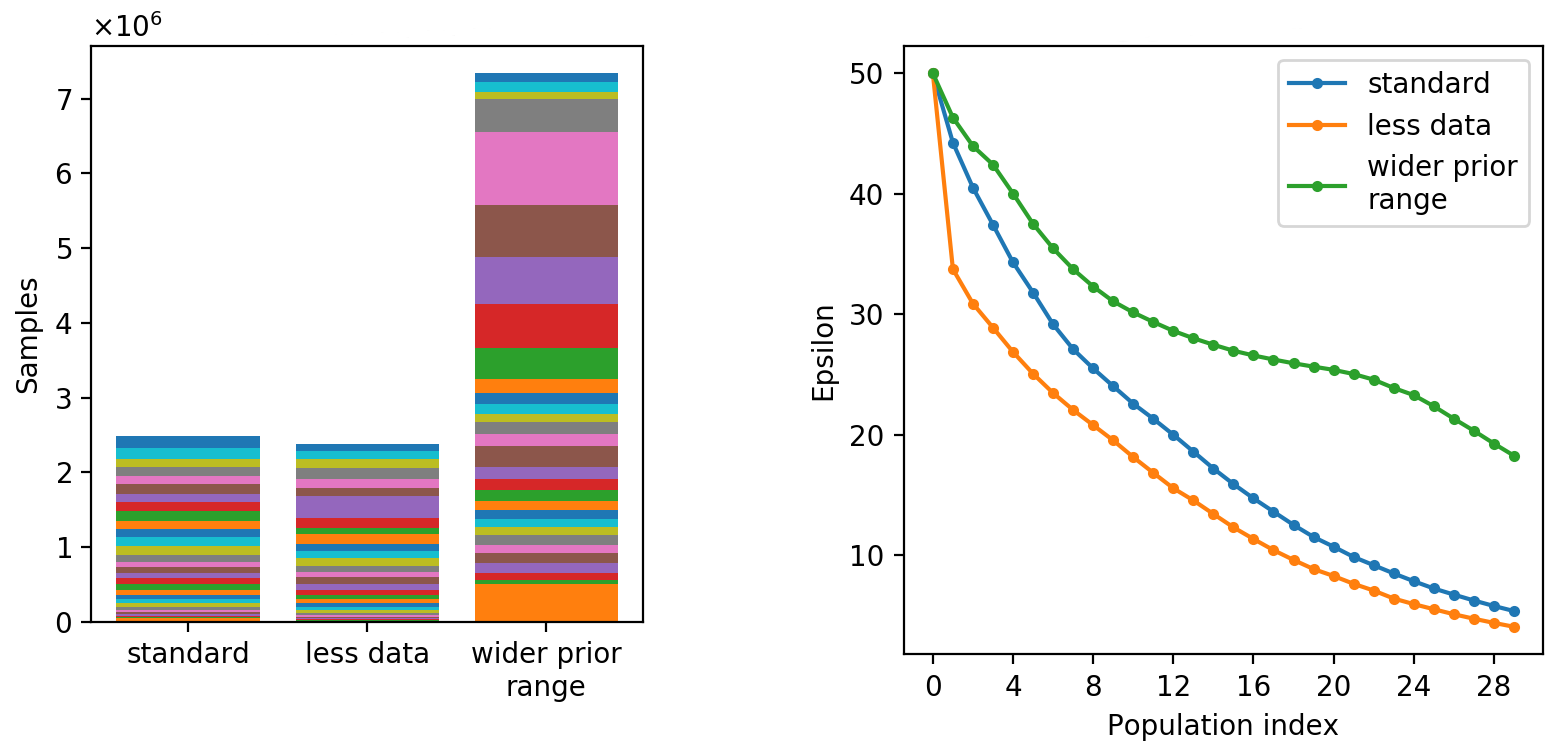
\includegraphics{fig/size1.png}}
    \end{center}
    
    \caption[Data size and prior distribution range experiment]%
        {Data size and prior distribution range experiment. (a) Total required samples, (b) Epsilon values under median epsilon schedule}
    \label{fig:size}
    
\end{figure}

[FIGURE HERE]


\subsubsection{Summary} This subsection aims to preliminarily explore ABC SMC settings using synthetic data with known true parameter values, thus the efficiency and the goodness of the resultant model can be compared across these options. Conclusion can be drawn to choose efficient and proper options of ABC SMC to be applied on the target models with experimental data. It also provides reference for a general inference task using SMC with high dimensional parameter space.








\section{Parameter estimation and model comparison}

\subsection{Model 1, 2 and 3}

[separated ABC run on model 1, 2 and 3]

Using the suggested options in the previous section, the target data (Figure \ref{fig:obs_data}) is prepared as input for the SMC inference framework. Regarding the result, the population size and number of generations are adjusted several times to obtain an general informative posterior which should be stable across repeated runs and avoid local optimal as much as possible.

Parameter estimation of model 1, 2 and 3 was tried with different prior distribution setting: distribution range [0, 25] and [0, 75], amd distribution type uniform and log-uniform. All these ABC SMC runs uses 2,000 particles per population and 30 generations. 

Log-uniform-shaped prior seems to give a better fit of the model, and wider prior range [0, 75] does not give a more accurate result. Then distribution range [0, 25] was tried, in case some parameter have a true posterior laying between [25, 50]. 

The results of prior distribution log-uniform [0, 50] is shown in Figure \ref{fig:result123}. For model 3, the acceptance rates and epsilon path are presented in Figure \ref{fig:result123_2}. For model 3, the estimated parameters' posterior is shown in Figure \ref{fig:para1}. Figure \ref{fig:result123} plots the estimated curve of models, using the mean value of each parameter's approximated posterior; also 1000 particles (each particle is a parameter set) were sampled and used to generate simulated trajectories of the four variable, and the mean (blue) and 25th to 75th percentile range (grey) are calculated from the 1000 simulated data.

Before applying model comparison methods, some features of the three model can still be compared. From simulated curves, It can be seen that all the inter-quartile ranges are tight around the mean value curve, which indicates the approximated posterior are concentrated to some degree; the peak-shaped posterior distributions (Figure \ref{fig:para1}) agrees with this. All epsilon values converges to a steady level, and model 3 has a lower final epsilon value and consequently the simulated trajectory is more close to the observed data (model 3, Figure \ref{fig:result123}).

The acceptance rates is fluctuating and have a gradually increase trend for all the three models, as the acceptance rate becomes higher when the true posteriors are gradually approximated. Compared to model 1, model 2 gives a better fit of the decreasing trend at the second half of the observed data, by using a exponentially decaying self-increase rate $\lambda_N$ instead of a constant. The resultant simulated data from model 2 and 3 are in the similar trends and the most obvious difference is that for model 3, the simulated data of $\Phi$ and $\alpha$ are more `flat'. We expect model 3 to be the best model as it reaches a threshold value and intuitively gives a better fit, although the fit could not be considered generally a good representation of the biological process that we want to model, as the simulated data are significantly biased from the observed data for tnf-$\alpha$. A sharp peak at 4 hpl is observed from the measurement (Figure \ref{fig:obs_data}) but no similar features are represented by any of the three models.

\begin{figure}
    \begin{center}
    \resizebox{1.0\hsize}{!}{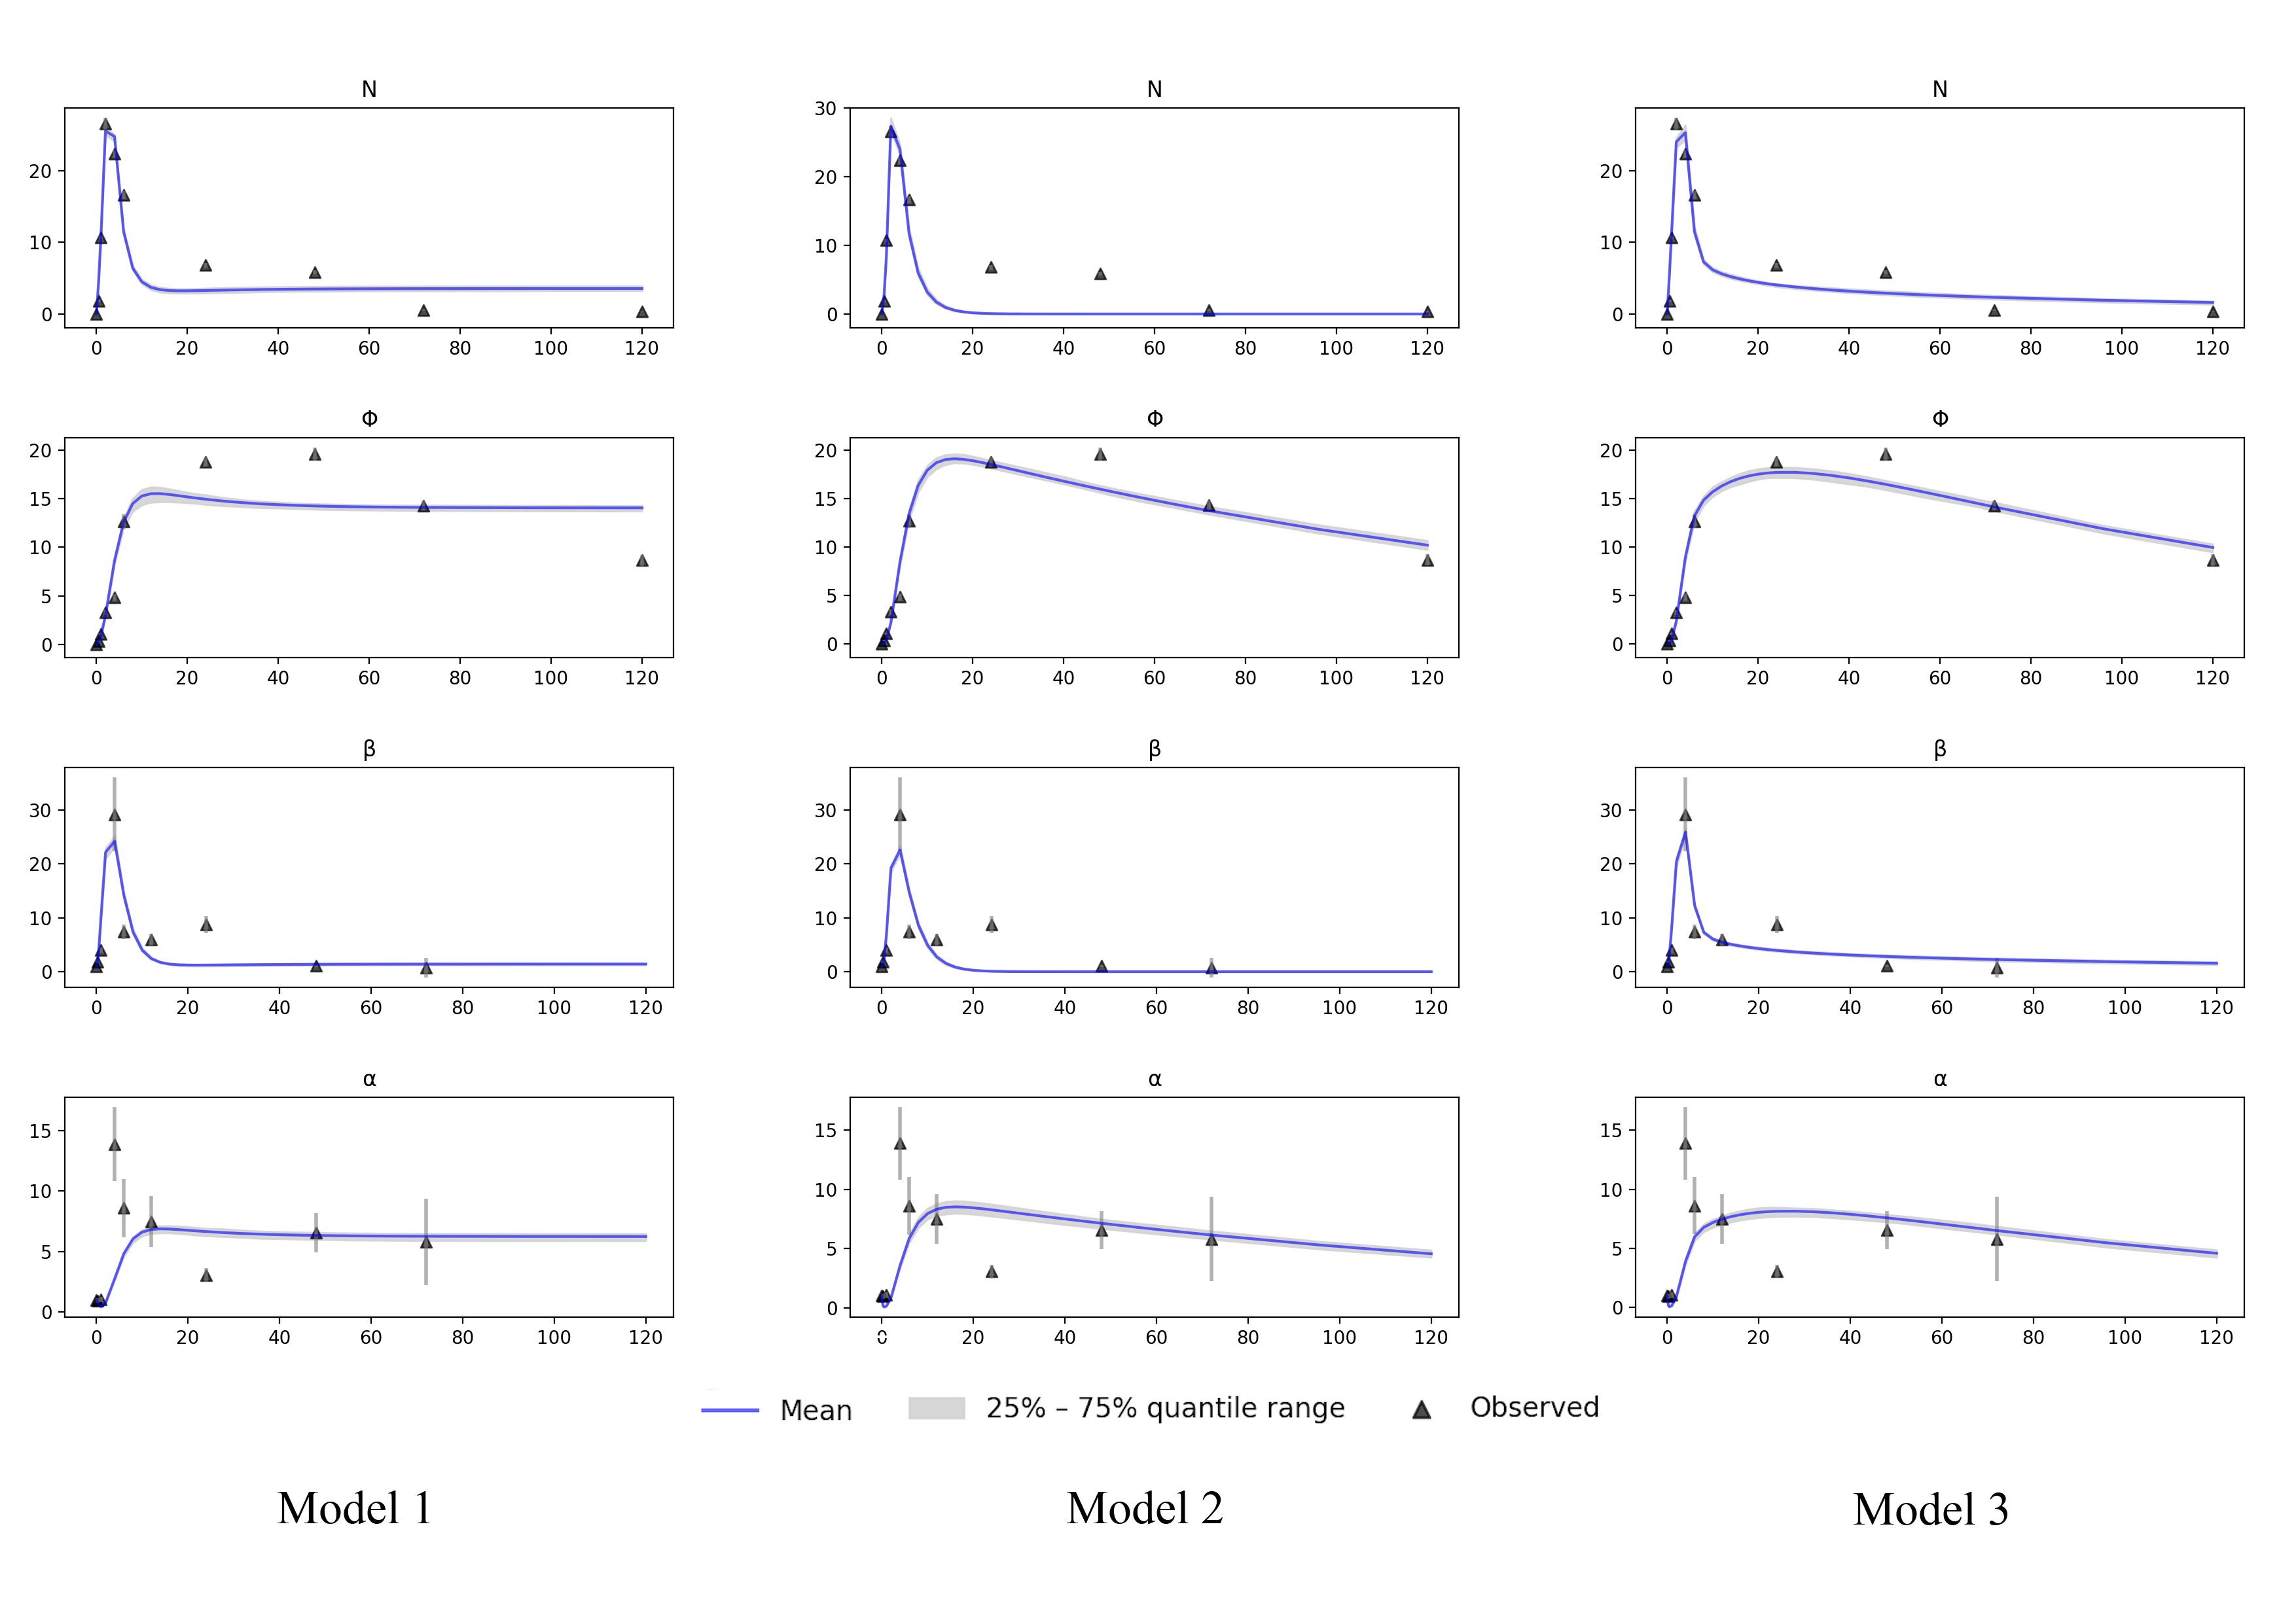
\includegraphics{fig/resultCurve123.png}}
    \end{center}
    
    \caption{Simulated trajectory from the last population of model 1, 2 and 3}
    \label{fig:result123}


    \vspace*{\floatsep}


    \begin{center}
        \resizebox{0.6\hsize}{!}{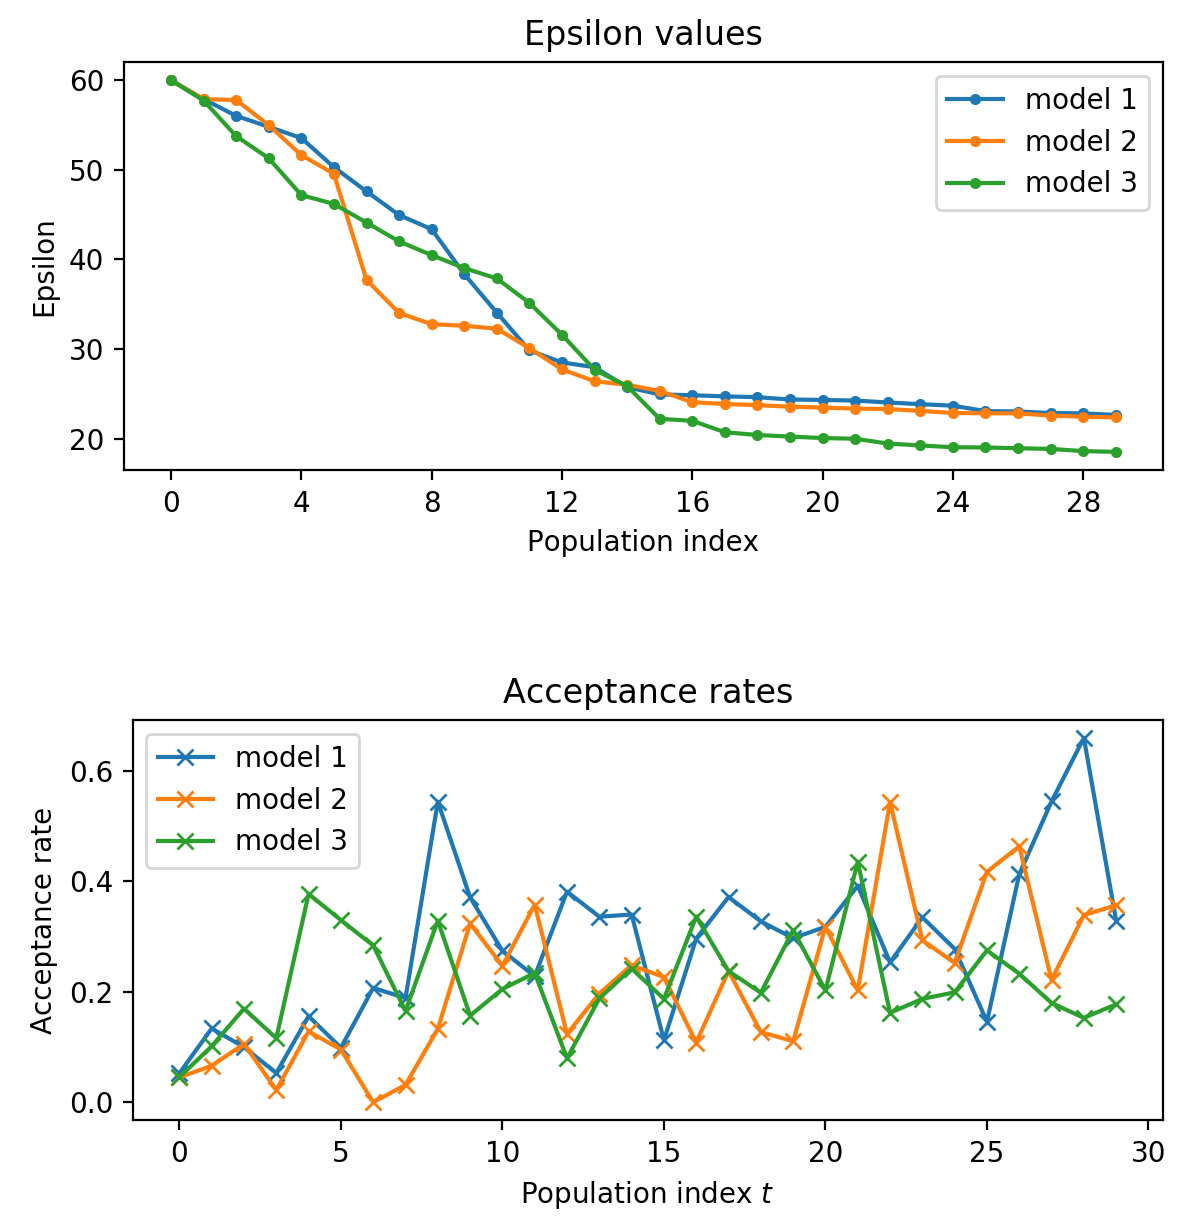
\includegraphics{fig/eps_acc123.png}}
        \end{center}
        
        \caption{Epsilon trends and acceptance rates of model 1, 2 and 3}
        \label{fig:result123_2}
    
\end{figure}

\begin{figure}
    \begin{center}
    \resizebox{1.0\hsize}{!}{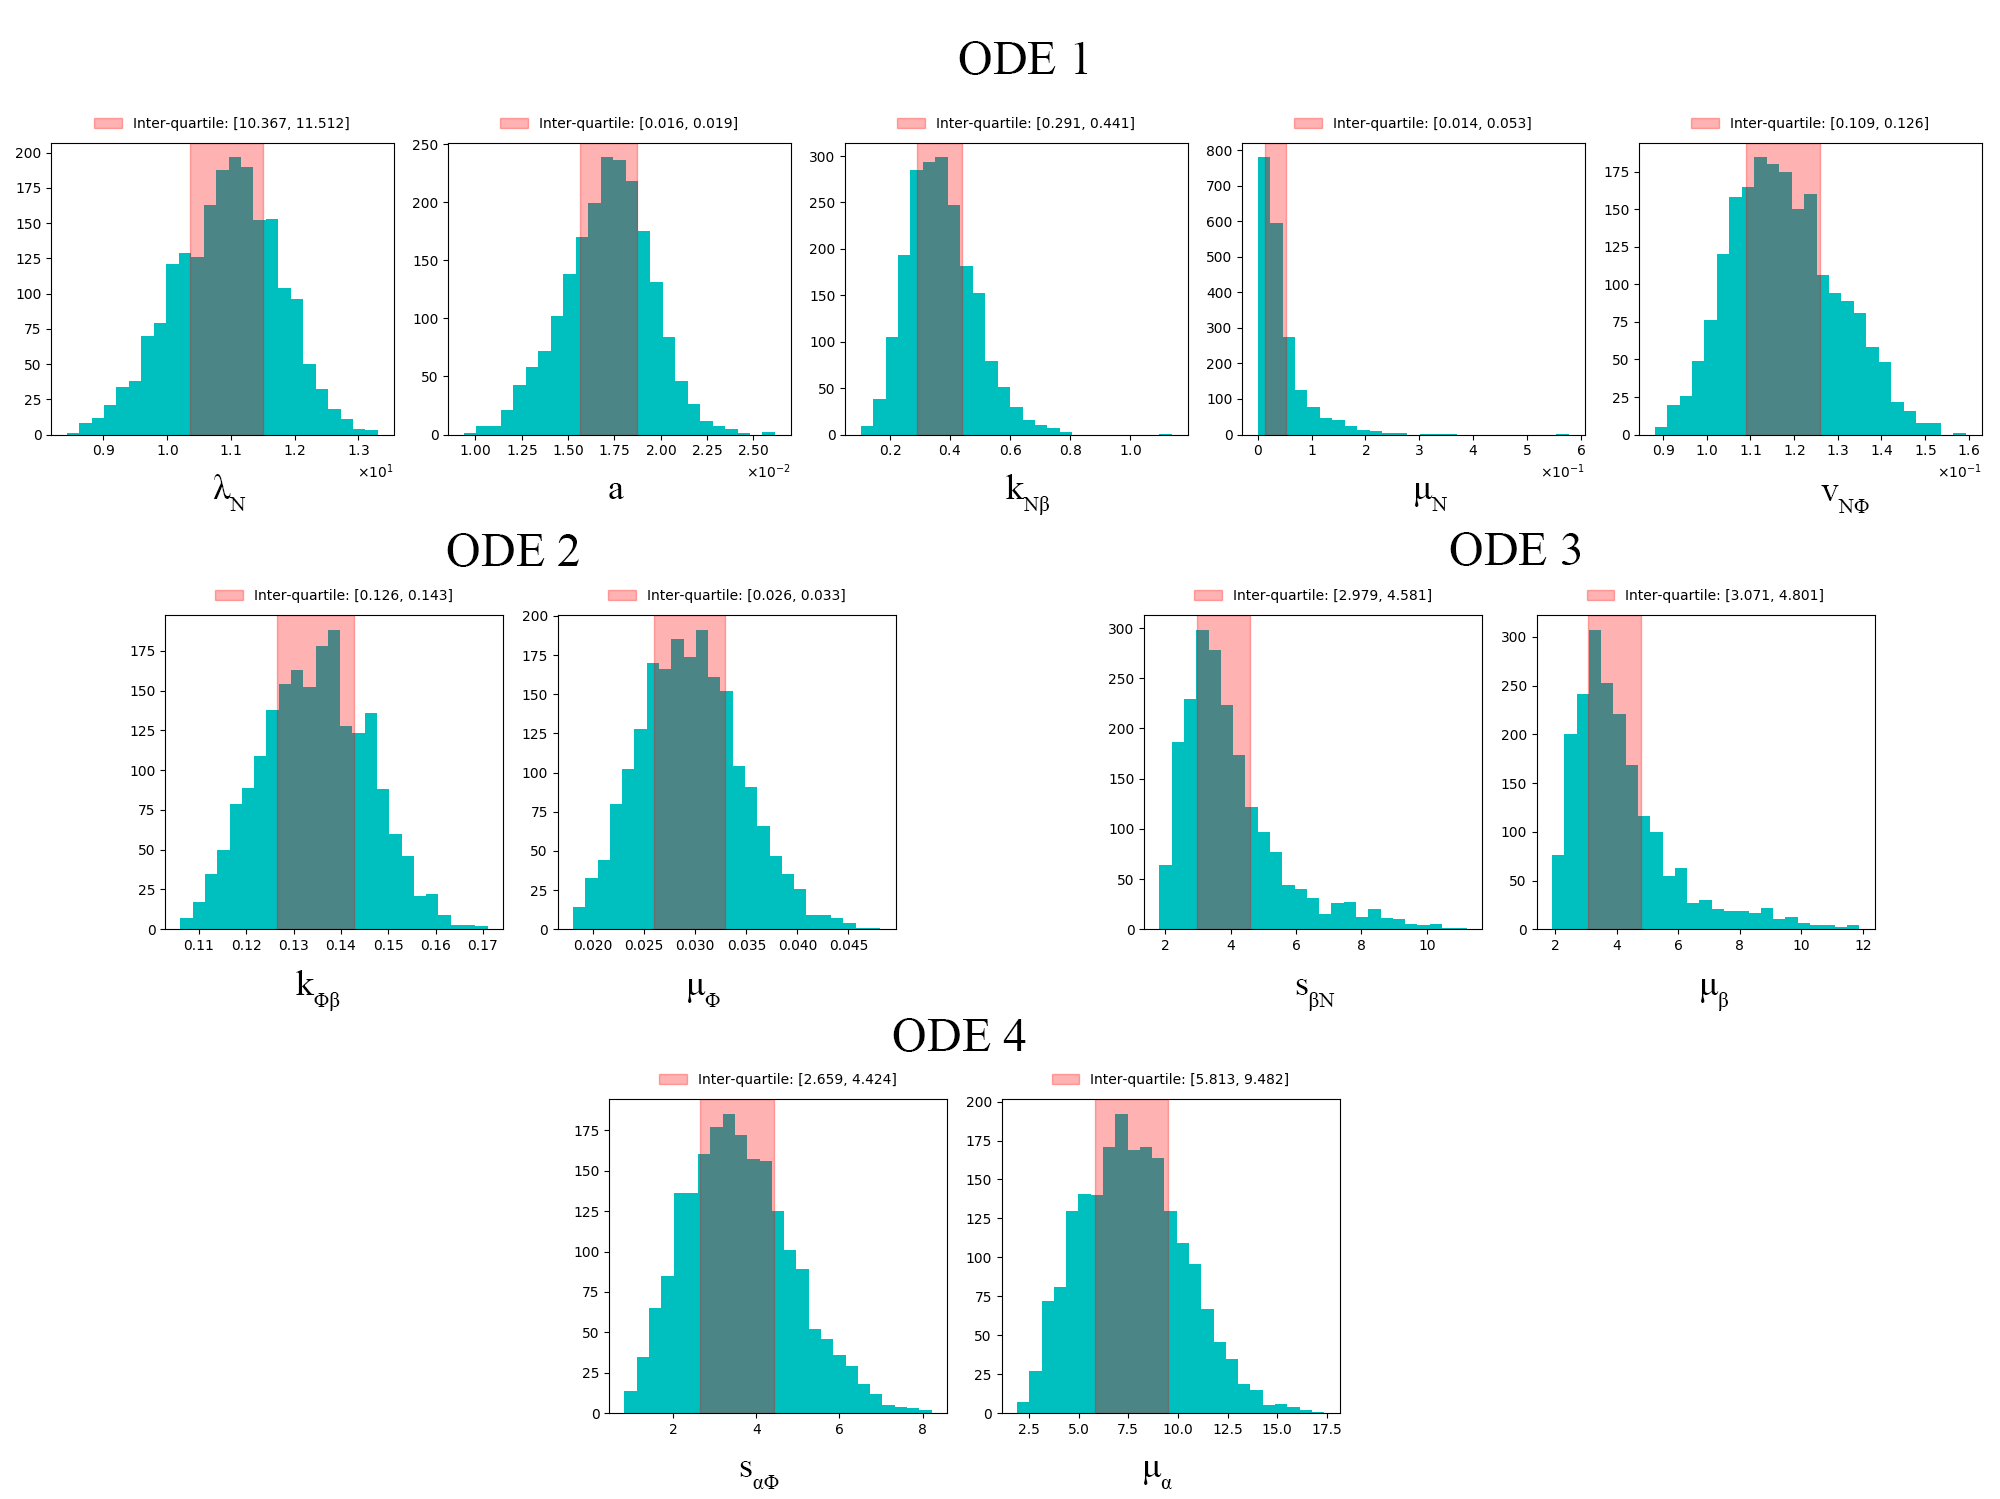
\includegraphics{fig/para1234.png}}
    \end{center}
    
    \caption{Estimated posterior distribution of parameters in model 3}
    \label{fig:para1}

    \begin{center}
        \resizebox{1.0\hsize}{!}{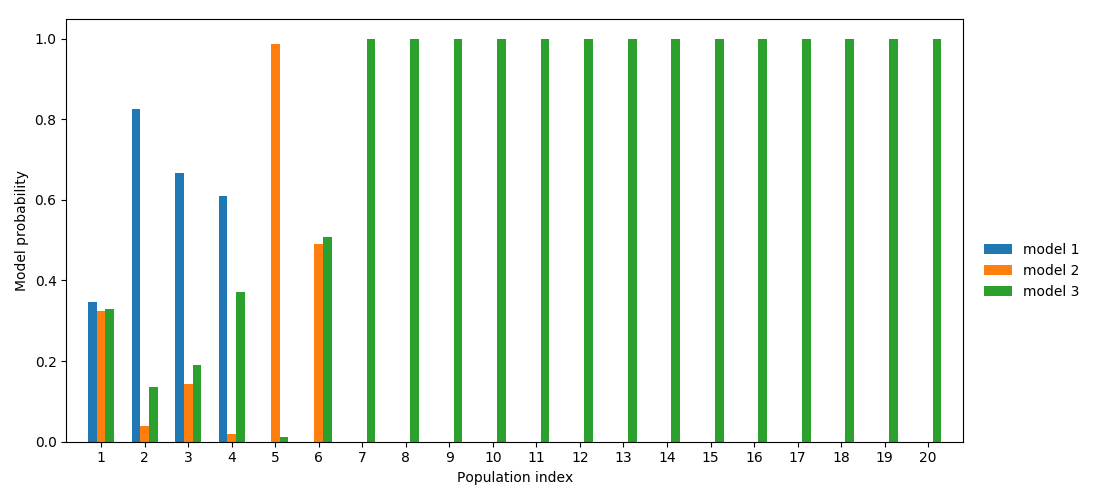
\includegraphics{fig/cmp1.png}}
        \end{center}
        
        \caption{Model comparison of model 1, 2 and 3}
        \label{fig:cmp1}
    
\end{figure}

[model comparison among model 1, 2, 3]

Next a model selection experiment with different prior was conducted, using the same ABC-SMC framework. As in the parameter inference, two distributions (uniform and log-uniform) are tested with three different interval ([0, 25], [0, 50] and [0, 75]). The results show that model 3 wins with nearly 100\% model probability at most runs after 30 generations, except log-uniform [0, 75]. All the model probability results are of great discrepancy (e.g. 100\% model 3 and 0\% for model 1 and 2), so Bayesian factor is not calculated. 

Figure \ref{fig:cmp1} shows the model selection process, under log-uniform [0, 50] prior distribution. Model 3 gains total advantage over model 1 and 2 after 7th population. Together with conclusions above, model 3 is considered to be the the best model to represent the target data so far.
 


\begin{table}[t!]
    \centering
    \begin{tabular}{|c c c|} 
     \hline
     Parameter & Estimated mean  & Estimated mean  \\ 
      & value (uniform) &value (log-uniform) \\[0.5ex] 
     \hline\hline
     $\lambda_N$ & 14.156 & 13.296  \\ 
     $a$ & 9.670 & 0.017  \\ 
     $\kappa_{N\beta}$ & 18.001 & 0.259 \\
     $\mu_N$ & 13.196 & 0.018 \\
     $\nu_{N\Phi}$ & 0.742 & 0.131 \\
     \hline
     $\kappa_{\Phi\beta}$ & 0.239 & 0.156 \\
     $\mu_\Phi$ & 0.154 & 0.035 \\
     \hline
     $s_{\beta N}$ & 6.752 & 1.213 \\
     $\mu_\beta$ & 6.378 & 1.315 \\
     \hline
     $s_{\alpha\Phi}$ & 16.997 & 5.826 \\
     $\mu_\alpha$ & 11.859 & 2.434\\
     \hline
    \end{tabular}
    \caption{Estimated parameter values of model 3}
    \label{table:estimated1}
\end{table}

Compared to uniform distributed prior, we found that log-uniform distributed prior is more suitable in the inference. Log-uniform results in an obviously better fit and narrower inter-quantile interval (Figure \ref{fig:result123} and \ref{fig:resultCurve_uni}), and the final epsilon value is also smaller. Log-uniform tends to assign values that are close to the left boundary (i.e. zero in our case) higher density, i.e. they are more likely to be sampled in the first population. As a result, the estimated parameter posteriors are expected to have smaller mean and/or skewed to left of the x-axis. The estimated values proved this (see \ref{table:estimated1}; also observed in other models and prior interval experiments). It indicates that some of the true parameter tend to have small values that are close to zero, and using log-uniform distribution could results in a faster and more satisfying inference. Regarding this, further experiments all use log-uniform distribution only.


\subsection{Model 4 and 5}

[features that derive model 4 and 5]

We observed that the existing models cannot well represent the trajectory of relative expression of tnf-$\alpha$: from experimental data, a rapid increase of tnf-$\alpha$ expression is observed in 0--4 hpl, followed by a rapid drop; all the models cannot well recover this feature and most test results see a less-rapid increase followed by a gradually decree and the observed peak value is not reached (e.g. Figure \ref{fig:result123}). Also in some other case e.g. Figure \ref{fig:resultCurve_uni}, tnf-$\alpha$ trajectories is well fitted at the cost of under-fitting $\Phi$. Hence efforts had been spent to propose more alternative models that can possibly solve this problem.

The two proposed alternative models is based on model 3 and try to add extra term in the tnf-$\alpha$ equation $\mathrm{d} \alpha/\mathrm{d} t$. As macrophage is the main source of tnf-$\alpha$ production, and a similar sharp increase-and-drop trend is observed in the il-1$\beta$ trajectory, two hypothesis and corresponding terms are propose as follows.

\paragraph{Model 4} It is assumed that the expression of il-1$\beta$ would have a promoting effect, representing by a phenomenological term $d_{\beta\alpha}\beta$ and $d_{\beta\alpha}$ is a new model parameter (positive constant). The promoting effect here is regarded to have the equivalent effect as directly promoting by il-1$\beta$, but the underlying mechanism is unclear so far. In mathematical view, this additional term can accelerate the expression of tnf-$\alpha$ in the first few time points and help to recover the peak-shaped trajectory. The proposed model is written as Equation \ref{eq:model4}.

\paragraph{Model 5} Alternatively, we considered promotions to the tnf-$\alpha$ production, i.e. $s_{\alpha\Phi}\Phi$. It is assumed that il-$\beta$ could accelerate the production process. An additional term $f_{\beta\alpha}\beta$ is introduced to production rate, with $f_{\beta\alpha}$ being a new model parameter (positive constant). This model meets the biological context considering the source of tnf-$\alpha$. The proposed model is written as Equation \ref{eq:model5}.

[further comparison of model 3, 4 and 5]

Model 4 and 5 are base on model 3, so in this phase experiments of these three models are conducted for separately parameter inference and overall model comparison. Based on our experience in conducted experiments, we used the following setting for parameter inference:

\begin{itemize}
    \item population size: 2000 and 5000
    \item number of populations: 30 generations
    \item prior: [0, 50] log-uniform
    \item perturbation kernel: multivariate normal kernel
\end{itemize}

Factors (Equation \ref{dis_f}) are also tried to find if we can force the inference framework to give more importance on the first few data points. In this experiment, for each trajectory first 8 data points are assigned higher factors (0.75), and the rest 4 data points are assigned with lower factors (0.25). All these runs are conducted on remote machines and the output database files are retrieved form analysis.

Figure \ref{fig:resultCurve345} shows the simulated data from the inferred models, with population size 2000. It can be seen that the addressed problem in the trajectory of tnf-$\alpha$ is partially relieved in model 4 and 5: compared to model 3, a peak appears around 4 hpl; it can represent more features in the observed data and consequently the final reached epsilon (after 30 populations) is smaller than that of model 3, which proves that our proposed modifications in model 4 and 5 are helpful in recovering more features in observed data.

\begin{figure}
    \begin{center}
    \resizebox{1.0\hsize}{!}{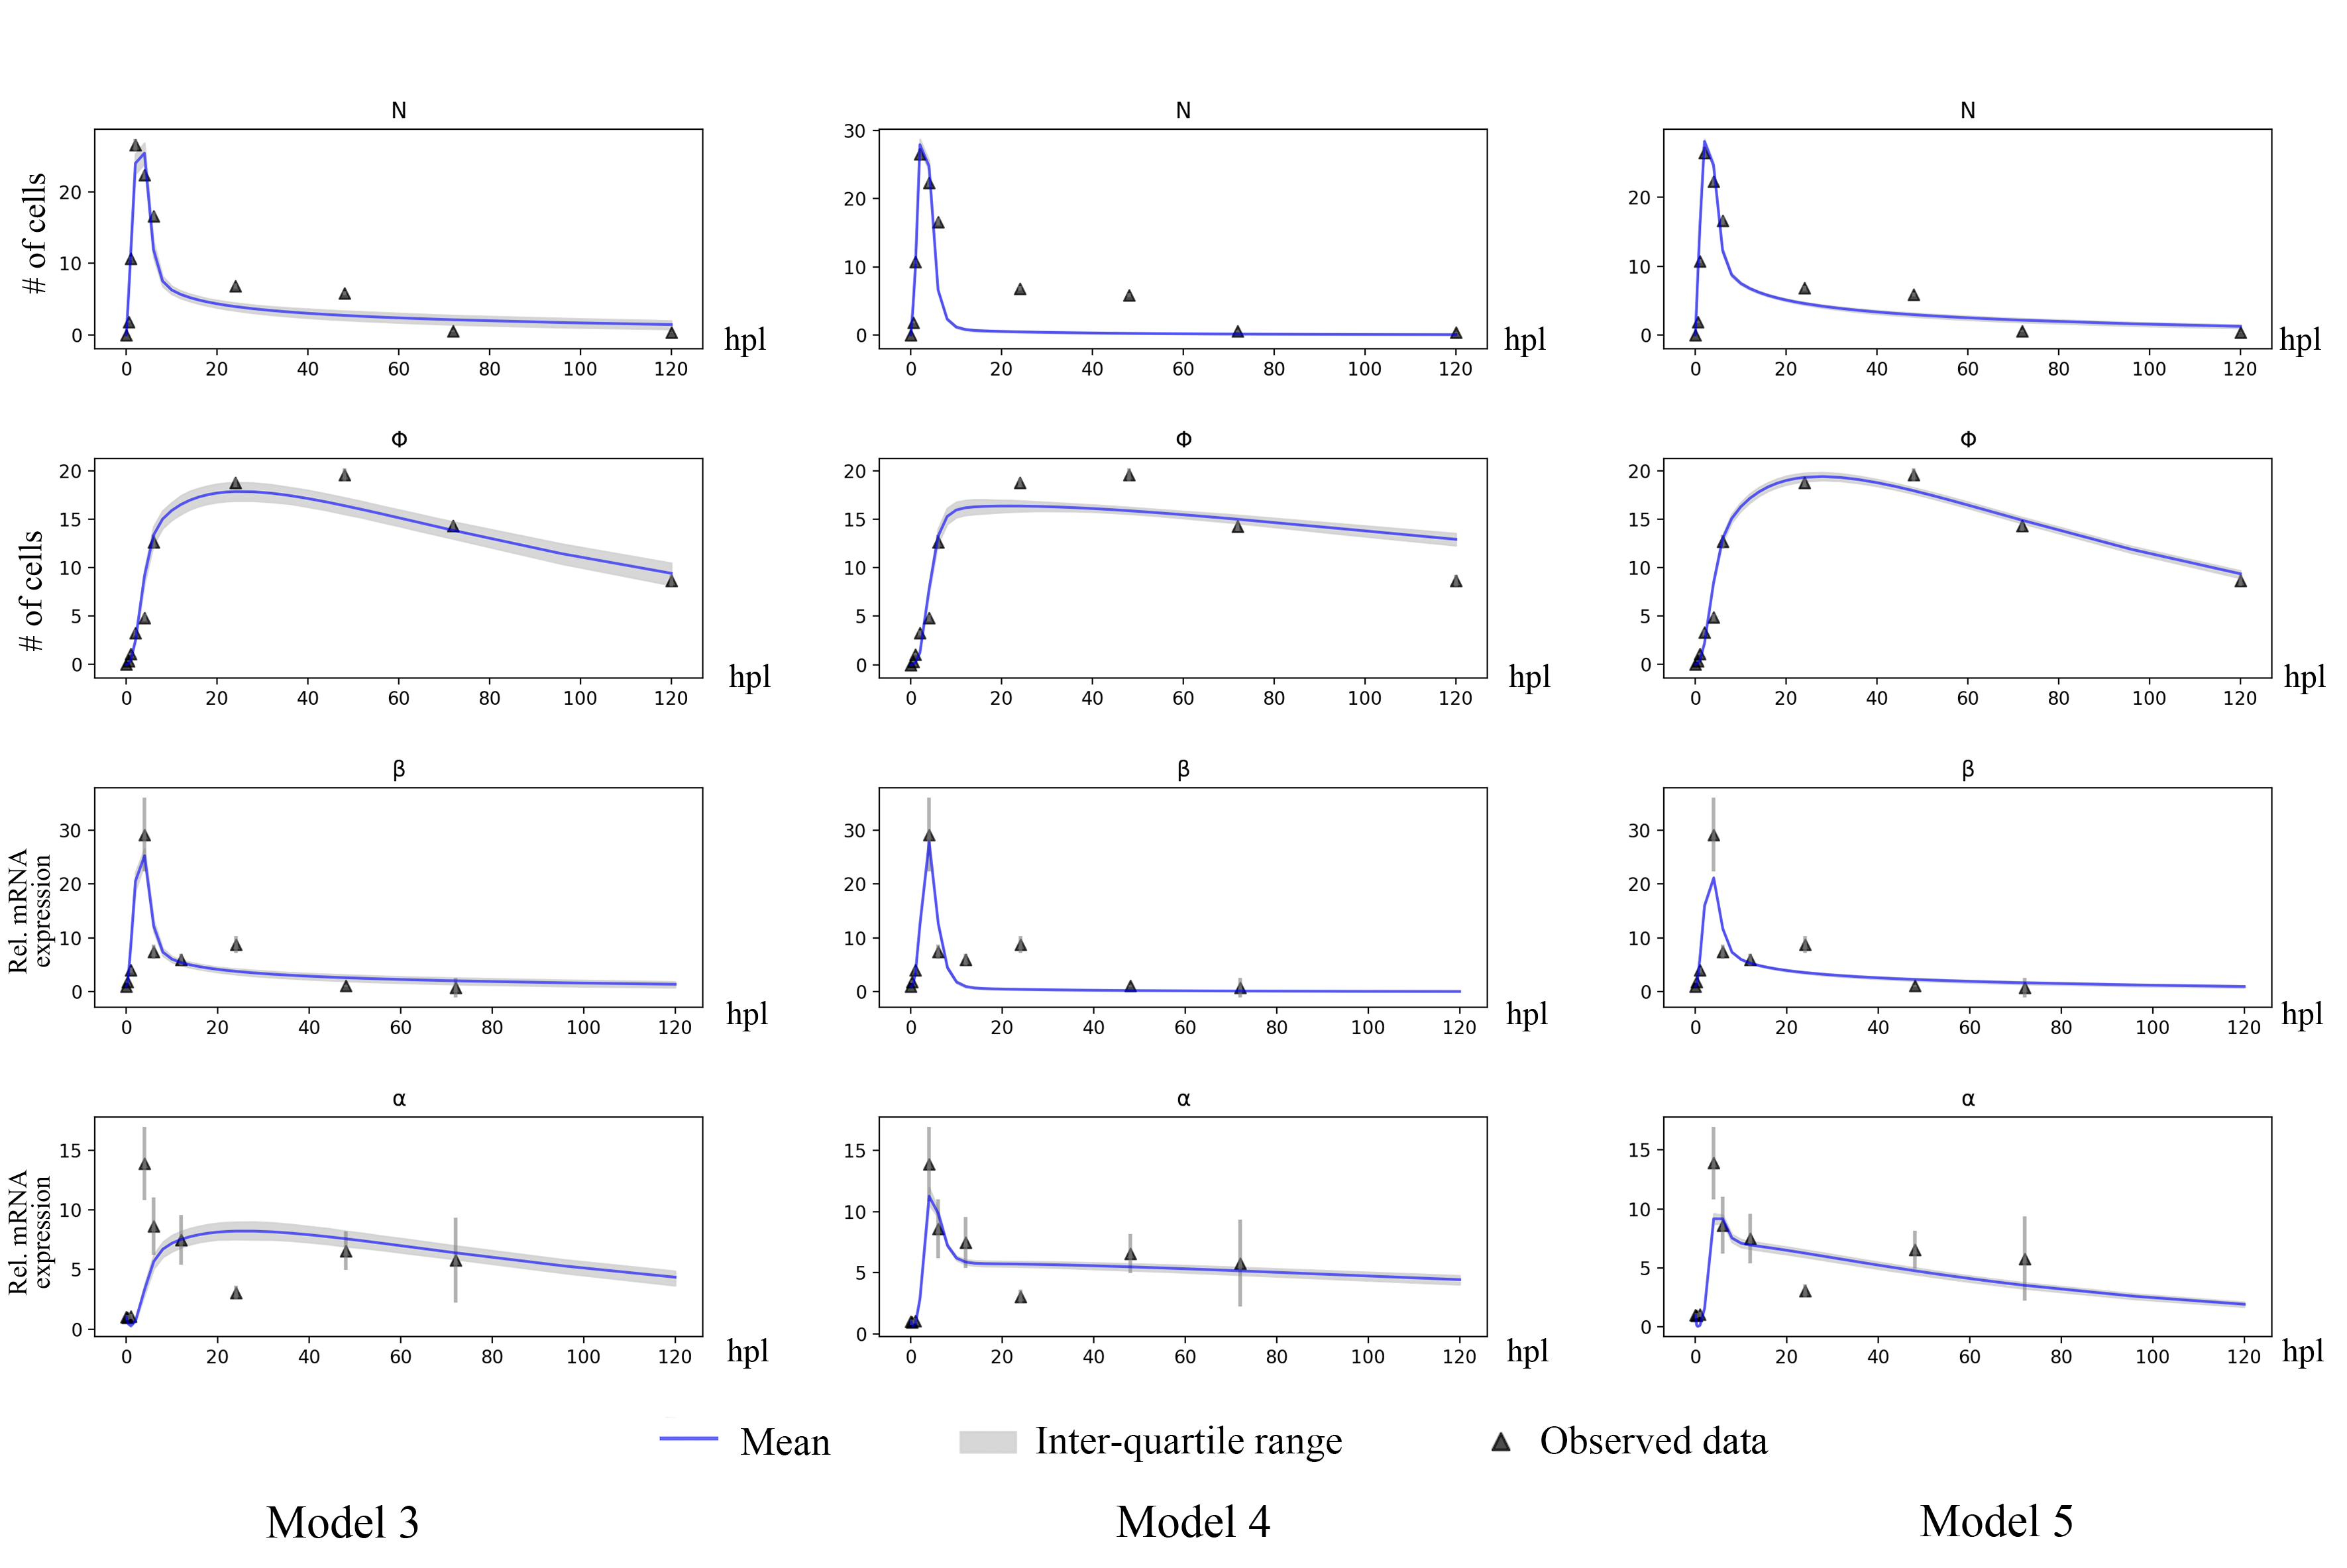
\includegraphics{fig/resultCurve345.png}}
    \end{center}
    
    \caption{Simulated data from the last population of model 3, 4 and 5}
    \label{fig:resultCurve345}
    
\end{figure}

By intuition model 4 and 5 would be the best models sofar that can recover most of observed data features. Model 1, 2 and 3 con also converge to a low final epsilon value (~20), but a key feature observed in target data -- a peak at around 4 hpl -- is not fitted. Some features, e.g. fluctuations in il-1$\beta$ and tnf-$alpha$ trajectories at around 20 hpl are still not ideally fitted; all existing models give a steady or gradually decrease trends for all the four variables after 20 hpl, and fluctuations in the observed data are fitted by smooth and steady curves.

After applying factors, the results were not largely different. As expected, applying factors made the data points at first half (where exists most of the fluctuations) more `focused', however the inferred models are close to one without factors, which could indicate that for model 4 and 5, applying factors will not largely affect the final convergency and the resultant posterior.

When we are trying more populations, an `over-fitting' behaviour is observed at the trajectory of macrophage (FIGURE). In this case, the discrepancy of simulated data and observed data comes from the last 2 data point (72 hpl and 120 hpl). 

Next, we performed a model selection on model 3, 4 and 5. FIGURE shows the model probabilities at different generations. From population 10 to population 20 model 4 gains advantage but after population 20 model 5 is preferred. Again, as DISCUSSED in the model comparison of model 1, 2 and 3, we considered the the violently changing model probability is related to the inference ability at certain epsilon threshold values (epsilon) and possibly the insufficient exploration of the parameter space. Given the present result, model 5 is regarded as the best model. Some further experiments tried larger population size (10,000 particles per population) and more populations (36 populations), but the resultant model did not have a significantly better fit of the observed data, although much more computation resources are used.

A inferred parameter posterior distribution of model 5 is shown in FIGURE, the estimated mean values is shown in TABLE. SOME DESCRIPTION.


\subsection{Sensitivity of parameters}

[why last PCs]

[which parameters are most sensitive]

[compared to credible intervals plot]

[what does that mean]

A quick sensitivity analysis of the dynamical systems models can be quantified using principle component analysis (PCA) \cite{Toni}, where the first PCs corresponds to sloppy parameters while the last PCs corresponds to stiff parameters \cite{sensitivity}. PCA can only provide rough approximated sensitivity behaviour. As models 5 won in the model selection, a further interest is to explore the parameter-to-model sensitivity

FIGURE shows the results of PCA on the last population of inferred model5. The last PC (PC12) is mostly consists of the linear combination of $a$ (from the equation of neutrophil) and $\mu_\Phi$ (from the equation of macrophage), to which the model is most sensitive. If we conclude the last 5 PCs (FIGURE), then $v_{N\Phi}$, $\mu_N)$ (from the equation of neutrophil) and $k_{\Phi\beta}$ (from the equation of macrophage) contribute most portions together with $a$ and $\mu_\Phi$. As a conclusion, model 5 is sensitive to changes in the above parameters, which all come from the equation of neutrophil and macrophage i.e. equations of the cells; it may suggests that given the observed data, the inferred model is more sensitive to cells' dynamic rather than cytokines' dynamics.

Also, some visualisations of the last population agreed with conclusions from PCA. Approximated posteriors of the last population plotted in FIGURE and credible ranges of parameters across populations in FIGURE shows that the 5 parameters identified by PCA is indeed `stiff' parameters.












\chapter{Performance experiments}

The performance experiments were designed to explore the parallel performance of ABC SMC inference framework which were used in the parameter estimation and model selection tasks. Usually ABC SMC is a time-consuming and computation intensive task and ideally executed on large clusters. The scheduling strategy, implementation details and many other factors can affect the parallel efficiency.

[MORE meanings of the performance study]

\section{Scaling-up}

First experiments are designed to illustrate the scaling-up performance. The program used here is an implementation of ABc SMC on model 5. The details of the ABC SMC settings is listed below

\begin{itemize}
    \item Prior distribution: default to log-uniform distribution [$1\times 10^{-6}$, 50] for all the 12 parameters
    \item threshold schedule: median epsilon
    \item No factors, no adaptive distance or adaptive population applied
    \item Population size is 2000, with 20 generations
\end{itemize}

[HOW PYABC parallelise the sampling]

For HPC systems like Cirrus, \verb|pyabc| uses \verb|multiprocessing| for multi-core parallel sampling. By default if the number of cores is not specified, it will automatically read the number of available cores and use them all. Cirrus has a 36-core CPU which support hyperthreading, such that the maximal number of cores available to \verb|multiprocessing| is 72.

The program is executed on Cirrus, using 8, 16, 24, 36, 54 and 72 cores respectively. Each run is repeated 10 times. The average execution time, required sampling numbers are recorded. Hyperthreading is enabled when using 54 and 72 cores. The access to the node that contains computation cores is exclusive, such that the execution would not be affected by other programs of operations.

The implementation of ABC SMC in \verb|pyabc| enables the parallelisation of sampling, which is the must time-consuming part. The rest part of the program is mostly not parallelised, e.g. database I/O and reductions operations. The sampling process involves sampling, perturbation and test of the acceptance criteria, all of which are computation-intensive. 

In practice, using ABC SMC to estimate the parameters of a given model could cost up to several hundred of hours if the computational resources is limited[REF]. The performance experiment result could provide a reference that illustrate that how the efficiency changes when scaling-up or the trade-offs in computational resources' cost and their benefit.

\subsubsection{Results}

[scaling-up performance: speed-up and efficiency]

[large variation in required sampling numbers]

[possible reasons]

The recorded execution time using different number of cores is shown in FIGURE. According to that, speed-up and efficiency can be calculated. Here 8 cores is regarded as the baseline for speed-up and efficiency, as the serial version (using only one core) can take quite a long time to finish 10 repeats. When increasing number of cores, the execution time drops fast at first but the decreasing rate (dropping speed, i.e. the derivative of the execution time against time) is gradually reduced to zero; 36, 54 and 72 cores gives nearly the same average execution time and consequently gains very close speedup values (FIGURE). 

Denote the number of cores used in the ABC SMC runs as variable $p$. The speedup curve shows a linear trend when $p\leq 36$; when $p\geq 36$ the speedup stays nearly unchanged. $p=36$ is an inflection point, where 36 is the maximum numbers available physical cores in a compute node of Cirrus. A constant drop of efficiency is observed when increasing $p$; smaller $p$ ($p<36$) gives an efficiency higher than 65\% but greater $p$ e.g. $p=72$ results in a low efficiency (34\%).

A high variance of total required samples was observed in the scaling-up experiments: some single runs required much more samples to finish 20 populations. Moreover, we found that the execution time is not ideally proportional to the total required samples (FIGURE). A possible explain to these phenomenons can be that the median epsilon schedule results in different threshold strategies due to the randomness in the sampling process, thus results in different approximate convergency paths for different runs. Some runs that are stuck in a local optimum and require smaller target epsilon will take huge amount of samples to move away from the local optimum. This have been observed when the distribution of posterior is plotted before and after jumping away from local modes (FIGURE and more explain). Also, time spent in each sample using sanme number of cores is not constant in our case, which might be a result of the parallel schedule; ideally a serial run using only one core will see a nearly constant time spent in every particle.

Due to the unstable sampling numbers, our interests switched to the per-particle performance, where the average sampling numbers per second (FIGURE) and average time spent in one particle (FIGURE) under different of cores ($p$) are plotted. The log-like average time per particle curve shows that using more cores can improve the sampling efficiency, but when $p$ is at a high level (e.g. 36 in our case), the improvement will be less significant.

\section{Profiling}

The performance could also be analysed given a profiling report. The second experiment profiles the program to reveal the detailed time consumption for each operation and the possible bottleneck, according to which we could find the hot-spot of program and given possible suggestions on improving the performance. 

In this case, profile tools \verb|cProfile| and \verb|yappi| is used in PyCharm IDE.

\subsubsection{Results} 

[profiling results: hot-spot and possible improvements]










% \chapter{Results and Discussions}

% [WHAT results is outputted and WHAT topics are discussed]

% \section{ABC SMC results}

% [inferred parameters: joint distribution, estimated values and simulated trajectory for each models; sensitivity; features of the inferred model]

% [model selections result; bayes factor]



% \section{Discussions}

% [goodness of fit (evaluation); preferred models and effects of modification to basic model]

% [efficiency and trade-offs in scaling-up]

% [POSSIBLE: compare to exact inference; compared to other implementations]

% [limitations]










\chapter{Future works}

[something not done as scheduled]

[interesting topics to look inside]

[moving to generalisations]









\chapter{Conclusions}

[what is studied]

[to what extend]

[how good is the result]

[summary of the findings and advise]

[thanks]








\appendix
% the appendix command just changes heading styles for appendices.

\chapter{System and software environment}

\section{ABC SMC implementation}

\subsection{Local machine}

Local development machine is a Mac laptop, running on macOS 10.15.6. The environment of the development is listed in Table \ref{table:local_macine}.

\begin{table}[h!]
    \centering
    \begin{tabular}{|c c|} 
     \hline
     Environment & Version \\ [0.5ex] 
     \hline\hline
     $\lambda_N$ & 2.1989  \\ 
     $\kappa_{N\beta}$ & 3.9627  \\
     $\mu_N$ & 1.7219 \\
     $\nu_{N\Phi}$  0.2195 & $cell^{-1}\cdotp h^{-1}$ \\
     \hline
     $\lambda_\Phi$ & 1.3146  $cell/h$ \\
     $\kappa_{\Phi\beta}$ 0.1235 & $cell/(unit\cdotp h)$ \\
     $\mu_\Phi$  0.1454 & $h^{-1}$ \\
     \hline
     $s_{\beta N}$ &6.5536  $unit/(cell\cdotp h)$ \\
     $i_{\beta\Phi}$  1.7062 & $cell^{-1}$ \\
     $\mu_\beta$ &0.5212  $h^{-1}$ \\
     \hline
     $s_{\alpha\Phi}$  10.2416 & $unit/(cell\cdotp h)$ \\
     $\mu_\alpha$ 19.6642 & $h^{-1}$ \\
    [1ex] 
     \hline
    \end{tabular}
    \caption{Environment on local machine}
    \label{table:local_macine}
\end{table}

\subsection{Remote machine}

\begin{table}[h!]
    \centering
    \begin{tabular}{|c c|} 
     \hline
     Environment & Version \\ [0.5ex] 
     \hline\hline
     $\lambda_N$ & 2.1989  \\ 
     $\kappa_{N\beta}$ & 3.9627  \\
     $\mu_N$ & 1.7219 \\
     $\nu_{N\Phi}$  0.2195 & $cell^{-1}\cdotp h^{-1}$ \\
     \hline
     $\lambda_\Phi$ & 1.3146  $cell/h$ \\
     $\kappa_{\Phi\beta}$ 0.1235 & $cell/(unit\cdotp h)$ \\
     $\mu_\Phi$  0.1454 & $h^{-1}$ \\
     \hline
     $s_{\beta N}$ &6.5536  $unit/(cell\cdotp h)$ \\
     $i_{\beta\Phi}$  1.7062 & $cell^{-1}$ \\
     $\mu_\beta$ &0.5212  $h^{-1}$ \\
     \hline
     $s_{\alpha\Phi}$  10.2416 & $unit/(cell\cdotp h)$ \\
     $\mu_\alpha$ 19.6642 & $h^{-1}$ \\
    [1ex] 
     \hline
    \end{tabular}
    \caption{Environment on remote machine}
    \label{table:remote_macine}
\end{table}

\section{Data analysis}

\chapter{Data and settings}






\section{Infer-back experiments}

\subsection{Parameter values used to generate synthetic data}

\begin{table}[h!]
    \centering
    \begin{tabular}{|c c c|} 
     \hline
     Parameter & Value & Unit\\ [0.5ex] 
     \hline\hline
     $\lambda_N$ & 2.1989 & $cell/h$  \\ 
     $\kappa_{N\beta}$ & 3.9627 & $cell/(unit\cdotp h)$\\
     $\mu_N$ & 1.7219 & $h^{-1}$\\
     $\nu_{N\Phi}$ & 0.2195 & $cell^{-1}\cdotp h^{-1}$ \\
     \hline
     $\lambda_\Phi$ & 1.3146 & $cell/h$ \\
     $\kappa_{\Phi\beta}$ & 0.1235 & $cell/(unit\cdotp h)$ \\
     $\mu_\Phi$ & 0.1454 & $h^{-1}$ \\
     \hline
     $s_{\beta N}$ & 6.5536 & $unit/(cell\cdotp h)$ \\
     $i_{\beta\Phi}$ & 1.7062 & $cell^{-1}$ \\
     $\mu_\beta$ & 0.5212 & $h^{-1}$ \\
     \hline
     $s_{\alpha\Phi}$ & 10.2416 & $unit/(cell\cdotp h)$ \\
     $\mu_\alpha$ & 19.6642 & $h^{-1}$ \\
    [1ex] 
     \hline
    \end{tabular}
    \caption{Parameter values used for model 1}
    \label{table:m1}
\end{table}

\subsection{Kernel experiment: median epsilon schedule}

\begin{figure}[h!]

    \begin{center}
    \resizebox{1.0\hsize}{!}{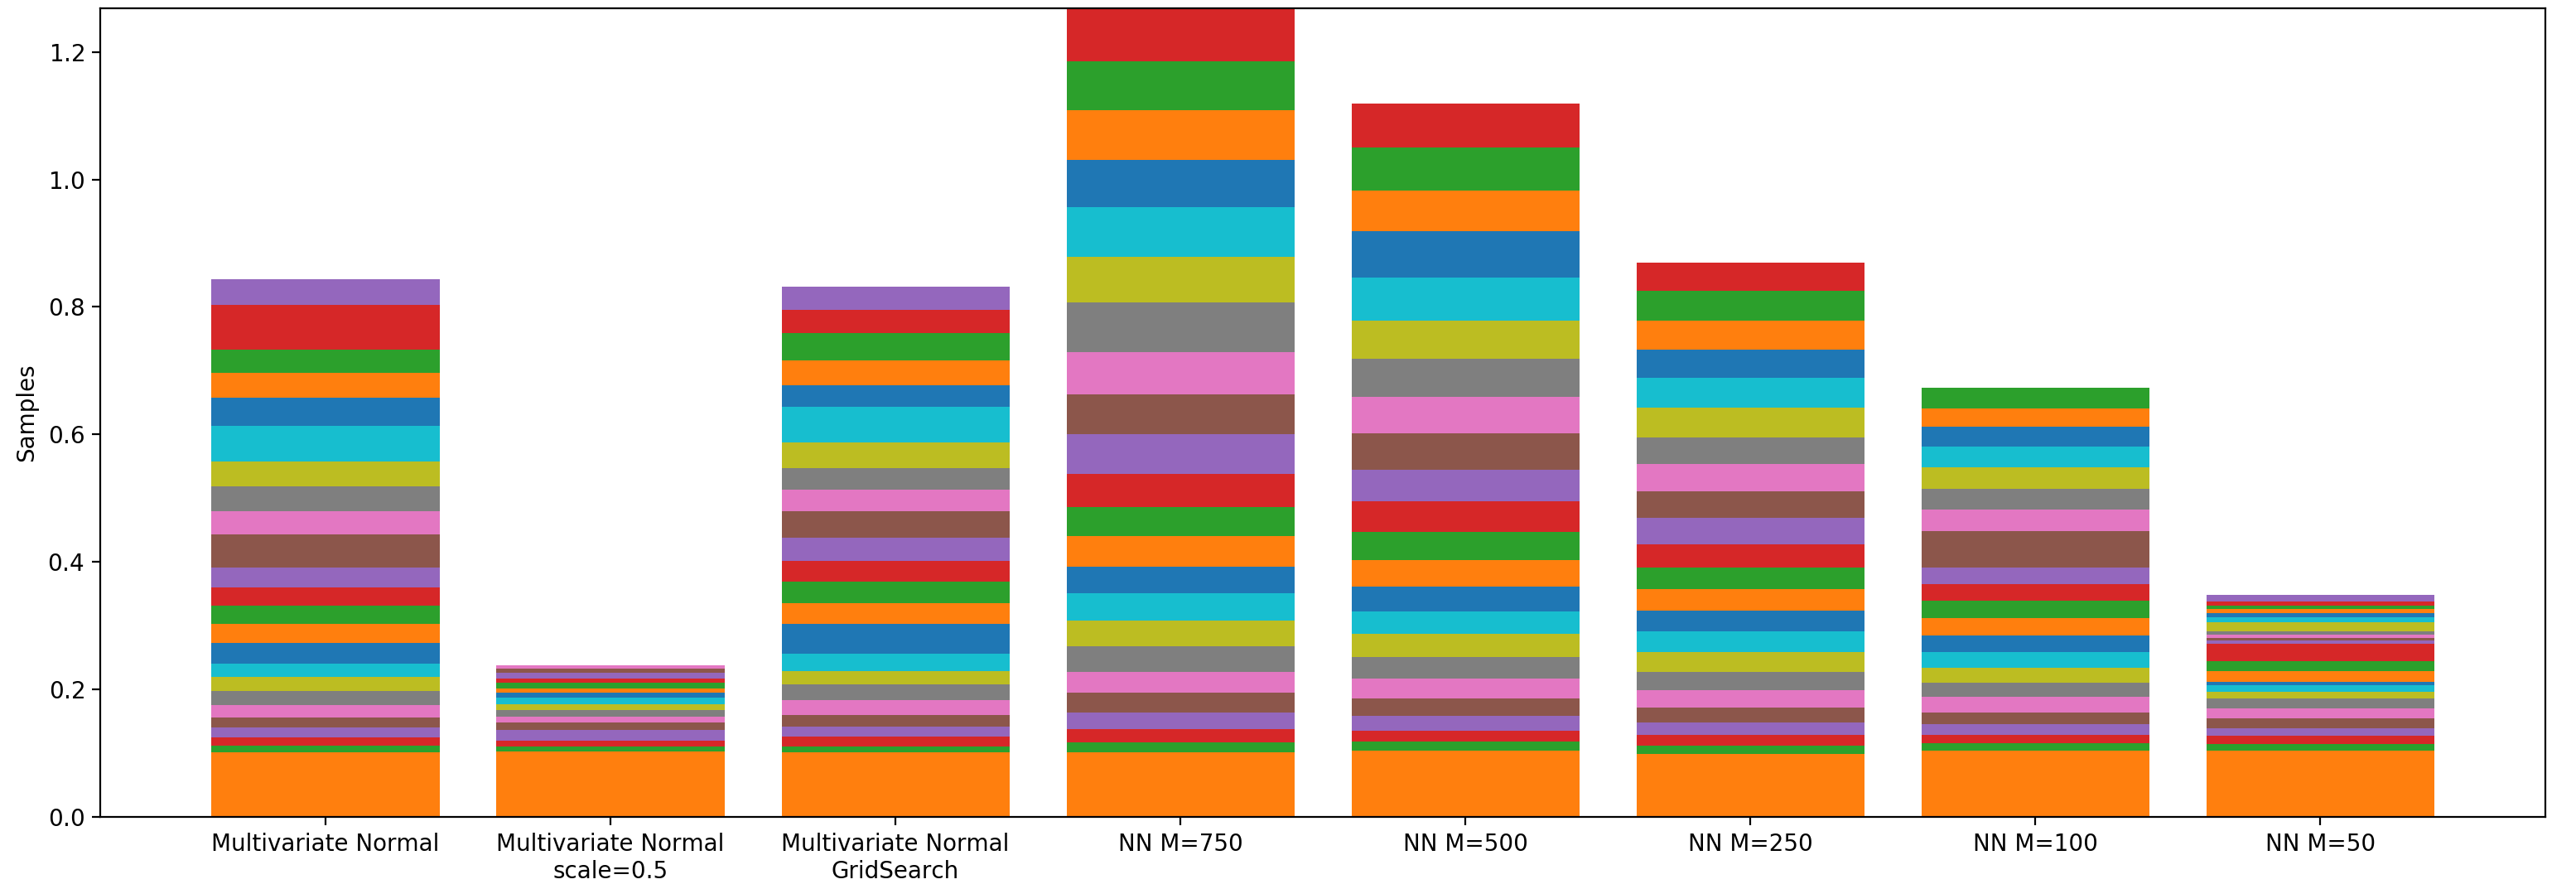
\includegraphics{fig/kernel2.png}}
    \end{center}
    
    \caption{Total sampling size} 
    \label{fig:kernel2}

    \begin{center}
        \resizebox{1.0\hsize}{!}{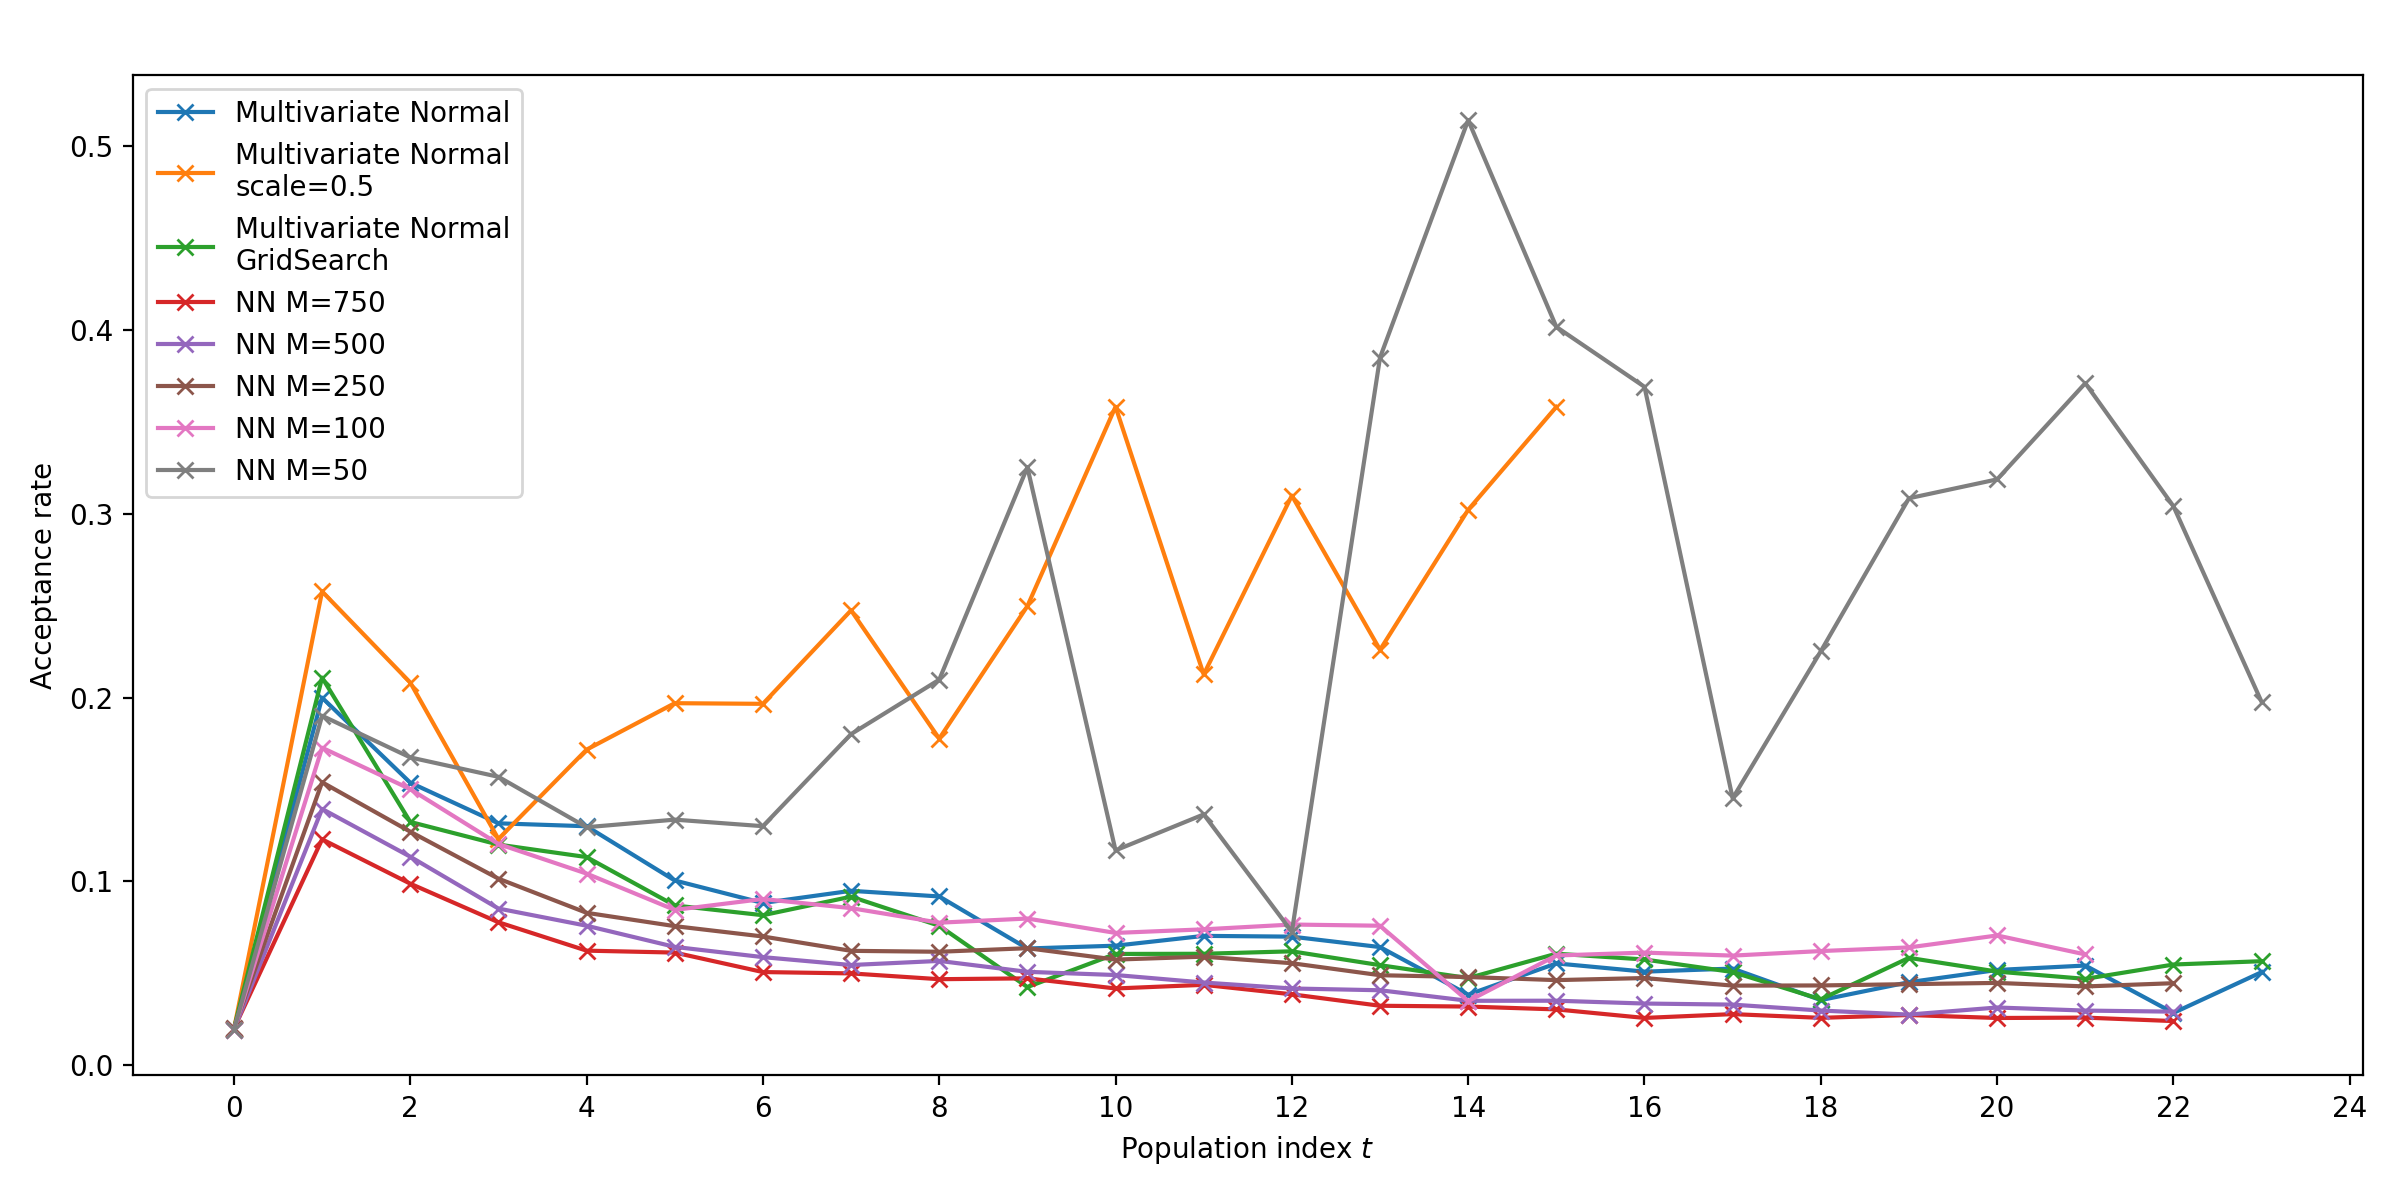
\includegraphics{fig/acceptance2.png}}
        \end{center}
        
        \caption{Acceptance rates} 
        \label{fig:acceptance2}
    
\end{figure}


\section{Parameter inference and model comparison results}

\begin{figure}[H]

    \begin{center}
    \resizebox{1.0\hsize}{!}{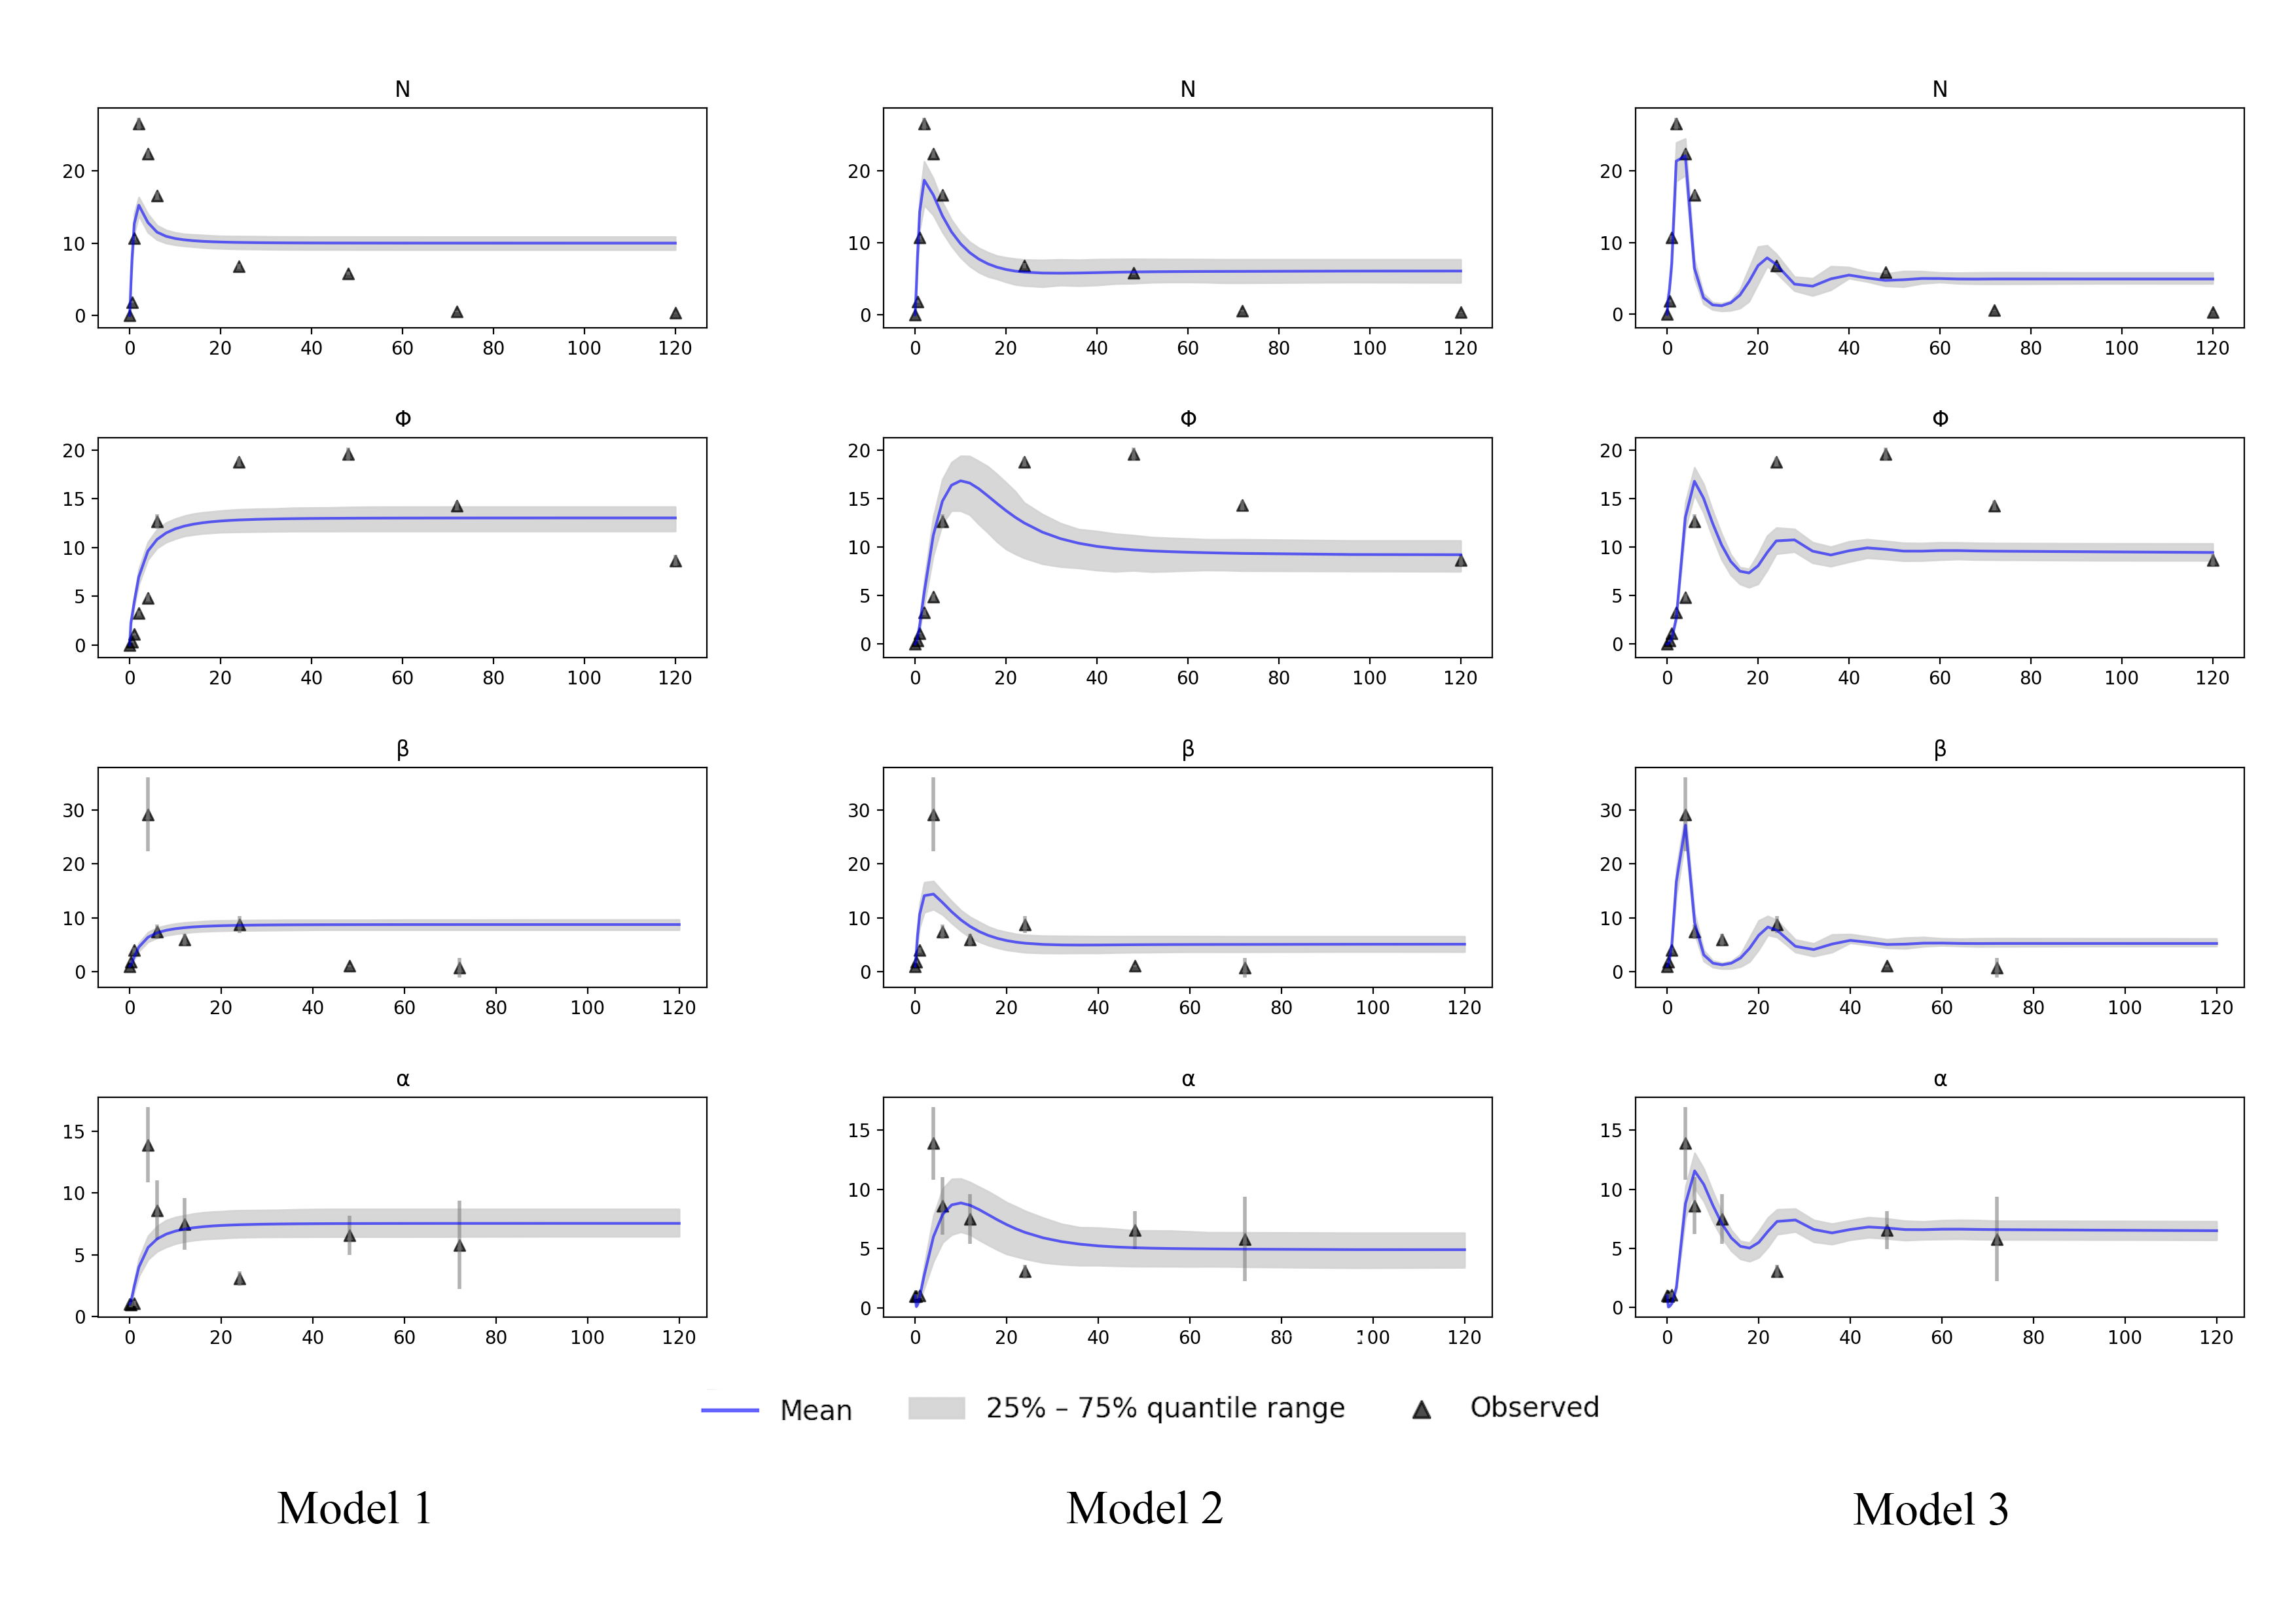
\includegraphics{fig/resultCurve_uni.png}}
    \end{center}
    
    \caption{Total sampling size} 
    \label{fig:resultCurve_uni}

    
\end{figure}












\begin{thebibliography}{100}

\bibitem{ref:Tsarouchas} Tsarouchas, T.M., Wehner, D., Cavone, L., Munir, T., Keatinge, M., Lambertus, M., Underhill, A., Barrett, T., Kassapis, E., Ogryzko, N. and Feng, Y., 2018. Dynamic control of proinflammatory cytokines Il-1$\beta$ and Tnf-$\alpha$ by macrophages in zebrafish spinal cord regeneration. Nature communications, 9(1), pp.1-17.

\bibitem{ref:pyabc} Klinger, E., Rickert, D. and Hasenauer, J., 2018. pyABC: distributed, likelihood-free inference. Bioinformatics, 34(20), pp.3591-3593.

\bibitem{ref:kernel} Filippi, S., Barnes, C. P., Cornebise, J., and Stumpf, M..H. (2013). On optimality of kernels for approximate Bayesian computation using sequential Monte Carlo. Statistical Applications in Genetics and Molecular Biology 12, 1, 87-107.

\bibitem{ref:abcsysbio} Liepe, J., Kirk, P., Filippi, S., Toni, T., Barnes, C.P., and Stumpf, M.P.H., 2014. A framework for parameter estimation and model selection from experimental data in systems biology using approximate Bayesian computation. Nature Protocols. 9 (2) pp. 439–456. 

\bibitem{ref:compare} Daly AC, Cooper J, GavaghanDJ, Holmes C. 2017. Comparing two sequentialMonte Carlo samplers for exact andapproximate Bayesian inference on biologicalmodels.J. R. Soc. Interface14: 20170340.

\bibitem{ref:disease} Minter, A. and Retkute, R., 2019. Approximate Bayesian Computation for infectious disease modelling. Epidemics, 29, p.100368.

\bibitem{ref:adpt_dis} Prangle, D., 2017. Adapting the ABC distance function. Bayesian Analysis, 12(1), pp.289-309.

\bibitem{ref:adpt_pop} Klinger, E. and Hasenauer, J., 2017, September. A scheme for adaptive selection of population sizes in approximate Bayesian computation-sequential Monte Carlo. In International Conference on Computational Methods in Systems Biology (pp. 128-144). Springer, Cham.

\bibitem{Toni} Toni, T., Welch, D., Strelkowa, N., Ipsen, A. and Stumpf, M.P., 2009. Approximate Bayesian computation scheme for parameter inference and model selection in dynamical systems. Journal of the Royal Society Interface, 6(31), pp.187-202.

\bibitem{sensitivity} Gutenkunst, R.N., Waterfall, J.J., Casey, F.P., Brown, K.S., Myers, C.R. and Sethna, J.P., 2007. Universally sloppy parameter sensitivities in systems biology models. PLoS Comput Biol, 3(10), p.e189.

\end{thebibliography}






\end{document}

